\documentclass[twoside]{book}

% Packages required by doxygen
\usepackage{fixltx2e}
\usepackage{calc}
\usepackage{doxygen}
\usepackage[export]{adjustbox} % also loads graphicx
\usepackage{graphicx}
\usepackage[utf8]{inputenc}
\usepackage{makeidx}
\usepackage{multicol}
\usepackage{multirow}
\PassOptionsToPackage{warn}{textcomp}
\usepackage{textcomp}
\usepackage[nointegrals]{wasysym}
\usepackage[table]{xcolor}

% Font selection
\usepackage[T1]{fontenc}
\usepackage[scaled=.90]{helvet}
\usepackage{courier}
\usepackage{amssymb}
\usepackage{sectsty}
\renewcommand{\familydefault}{\sfdefault}
\allsectionsfont{%
  \fontseries{bc}\selectfont%
  \color{darkgray}%
}
\renewcommand{\DoxyLabelFont}{%
  \fontseries{bc}\selectfont%
  \color{darkgray}%
}
\newcommand{\+}{\discretionary{\mbox{\scriptsize$\hookleftarrow$}}{}{}}

% Page & text layout
\usepackage{geometry}
\geometry{%
  a4paper,%
  top=2.5cm,%
  bottom=2.5cm,%
  left=2.5cm,%
  right=2.5cm%
}
\tolerance=750
\hfuzz=15pt
\hbadness=750
\setlength{\emergencystretch}{15pt}
\setlength{\parindent}{0cm}
\setlength{\parskip}{3ex plus 2ex minus 2ex}
\makeatletter
\renewcommand{\paragraph}{%
  \@startsection{paragraph}{4}{0ex}{-1.0ex}{1.0ex}{%
    \normalfont\normalsize\bfseries\SS@parafont%
  }%
}
\renewcommand{\subparagraph}{%
  \@startsection{subparagraph}{5}{0ex}{-1.0ex}{1.0ex}{%
    \normalfont\normalsize\bfseries\SS@subparafont%
  }%
}
\makeatother

% Headers & footers
\usepackage{fancyhdr}
\pagestyle{fancyplain}
\fancyhead[LE]{\fancyplain{}{\bfseries\thepage}}
\fancyhead[CE]{\fancyplain{}{}}
\fancyhead[RE]{\fancyplain{}{\bfseries\leftmark}}
\fancyhead[LO]{\fancyplain{}{\bfseries\rightmark}}
\fancyhead[CO]{\fancyplain{}{}}
\fancyhead[RO]{\fancyplain{}{\bfseries\thepage}}
\fancyfoot[LE]{\fancyplain{}{}}
\fancyfoot[CE]{\fancyplain{}{}}
\fancyfoot[RE]{\fancyplain{}{\bfseries\scriptsize Generated by Doxygen }}
\fancyfoot[LO]{\fancyplain{}{\bfseries\scriptsize Generated by Doxygen }}
\fancyfoot[CO]{\fancyplain{}{}}
\fancyfoot[RO]{\fancyplain{}{}}
\renewcommand{\footrulewidth}{0.4pt}
\renewcommand{\chaptermark}[1]{%
  \markboth{#1}{}%
}
\renewcommand{\sectionmark}[1]{%
  \markright{\thesection\ #1}%
}

% Indices & bibliography
\usepackage{natbib}
\usepackage[titles]{tocloft}
\setcounter{tocdepth}{3}
\setcounter{secnumdepth}{5}
\makeindex

% Hyperlinks (required, but should be loaded last)
\usepackage{ifpdf}
\ifpdf
  \usepackage[pdftex,pagebackref=true]{hyperref}
\else
  \usepackage[ps2pdf,pagebackref=true]{hyperref}
\fi
\hypersetup{%
  colorlinks=true,%
  linkcolor=blue,%
  citecolor=blue,%
  unicode%
}

% Custom commands
\newcommand{\clearemptydoublepage}{%
  \newpage{\pagestyle{empty}\cleardoublepage}%
}

\usepackage{caption}
\captionsetup{labelsep=space,justification=centering,font={bf},singlelinecheck=off,skip=4pt,position=top}

%===== C O N T E N T S =====

\begin{document}

% Titlepage & ToC
\hypersetup{pageanchor=false,
             bookmarksnumbered=true,
             pdfencoding=unicode
            }
\pagenumbering{alph}
\begin{titlepage}
\vspace*{7cm}
\begin{center}%
{\Large sqlite-\/api }\\
\vspace*{1cm}
{\large Generated by Doxygen 1.8.14}\\
\end{center}
\end{titlepage}
\clearemptydoublepage
\pagenumbering{roman}
\tableofcontents
\clearemptydoublepage
\pagenumbering{arabic}
\hypersetup{pageanchor=true}

%--- Begin generated contents ---
\chapter{sqlite-\/api}
\label{md_README}
\Hypertarget{md_README}
\input{md_README}
\chapter{Hierarchical Index}
\section{Class Hierarchy}
This inheritance list is sorted roughly, but not completely, alphabetically\+:\begin{DoxyCompactList}
\item \contentsline{section}{cmp\+\_\+str}{\pageref{structcmp__str}}{}
\item \contentsline{section}{Columns}{\pageref{classColumns}}{}
\begin{DoxyCompactList}
\item \contentsline{section}{Entity}{\pageref{classEntity}}{}
\begin{DoxyCompactList}
\item \contentsline{section}{U\+A\+T\+Data}{\pageref{classUATData}}{}
\end{DoxyCompactList}
\end{DoxyCompactList}
\item \contentsline{section}{Columns\+From\+Sql\+Value}{\pageref{classColumnsFromSqlValue}}{}
\item \contentsline{section}{DB}{\pageref{classDB}}{}
\item \contentsline{section}{Default\+Data\+Creation\+Policy}{\pageref{classDefaultDataCreationPolicy}}{}
\item Entity\+Creation\+Policy\begin{DoxyCompactList}
\item \contentsline{section}{Db\+Manager$<$ Entity\+Creation\+Policy $>$}{\pageref{classDbManager}}{}
\end{DoxyCompactList}
\item \contentsline{section}{Sql\+Factory}{\pageref{classSqlFactory}}{}
\item \contentsline{section}{Sql\+Field}{\pageref{structSqlField}}{}
\item \contentsline{section}{sqlite3\+\_\+deleter}{\pageref{structsqlite3__deleter}}{}
\item \contentsline{section}{sqlite3\+\_\+stmt\+\_\+deleter}{\pageref{structsqlite3__stmt__deleter}}{}
\item \contentsline{section}{Sql\+Value}{\pageref{structSqlValue}}{}
\item \contentsline{section}{Sql\+Value\+From\+Column}{\pageref{classSqlValueFromColumn}}{}
\item \contentsline{section}{Table}{\pageref{classTable}}{}
\item \contentsline{section}{U\+A\+T\+Domain\+Creation\+Policy}{\pageref{classUATDomainCreationPolicy}}{}
\end{DoxyCompactList}

\chapter{Class Index}
\section{Class List}
Here are the classes, structs, unions and interfaces with brief descriptions\+:\begin{DoxyCompactList}
\item\contentsline{section}{\mbox{\hyperlink{structcmp__str}{cmp\+\_\+str}} }{\pageref{structcmp__str}}{}
\item\contentsline{section}{\mbox{\hyperlink{classColumns}{Columns}} }{\pageref{classColumns}}{}
\item\contentsline{section}{\mbox{\hyperlink{classColumnsFromSqlValue}{Columns\+From\+Sql\+Value}} }{\pageref{classColumnsFromSqlValue}}{}
\item\contentsline{section}{\mbox{\hyperlink{classDB}{DB}} }{\pageref{classDB}}{}
\item\contentsline{section}{\mbox{\hyperlink{classDbManager}{Db\+Manager$<$ Entity\+Creation\+Policy $>$}} }{\pageref{classDbManager}}{}
\item\contentsline{section}{\mbox{\hyperlink{classDefaultDataCreationPolicy}{Default\+Data\+Creation\+Policy}} }{\pageref{classDefaultDataCreationPolicy}}{}
\item\contentsline{section}{\mbox{\hyperlink{classEntity}{Entity}} }{\pageref{classEntity}}{}
\item\contentsline{section}{\mbox{\hyperlink{classSqlFactory}{Sql\+Factory}} }{\pageref{classSqlFactory}}{}
\item\contentsline{section}{\mbox{\hyperlink{structSqlField}{Sql\+Field}} }{\pageref{structSqlField}}{}
\item\contentsline{section}{\mbox{\hyperlink{structsqlite3__deleter}{sqlite3\+\_\+deleter}} }{\pageref{structsqlite3__deleter}}{}
\item\contentsline{section}{\mbox{\hyperlink{structsqlite3__stmt__deleter}{sqlite3\+\_\+stmt\+\_\+deleter}} }{\pageref{structsqlite3__stmt__deleter}}{}
\item\contentsline{section}{\mbox{\hyperlink{structSqlValue}{Sql\+Value}} }{\pageref{structSqlValue}}{}
\item\contentsline{section}{\mbox{\hyperlink{classSqlValueFromColumn}{Sql\+Value\+From\+Column}} }{\pageref{classSqlValueFromColumn}}{}
\item\contentsline{section}{\mbox{\hyperlink{classTable}{Table}} }{\pageref{classTable}}{}
\item\contentsline{section}{\mbox{\hyperlink{classUATData}{U\+A\+T\+Data}} }{\pageref{classUATData}}{}
\item\contentsline{section}{\mbox{\hyperlink{classUATDomainCreationPolicy}{U\+A\+T\+Domain\+Creation\+Policy}} }{\pageref{classUATDomainCreationPolicy}}{}
\end{DoxyCompactList}

\chapter{File Index}
\section{File List}
Here is a list of all files with brief descriptions\+:\begin{DoxyCompactList}
\item\contentsline{section}{\mbox{\hyperlink{main_8cpp}{main.\+cpp}} }{\pageref{main_8cpp}}{}
\item\contentsline{section}{sqlite-\/core/\+Headers/\mbox{\hyperlink{columns_8h}{columns.\+h}} }{\pageref{columns_8h}}{}
\item\contentsline{section}{sqlite-\/core/\+Headers/\mbox{\hyperlink{databroker_8h}{databroker.\+h}} }{\pageref{databroker_8h}}{}
\item\contentsline{section}{sqlite-\/core/\+Headers/\mbox{\hyperlink{datadefinition_8h}{datadefinition.\+h}} }{\pageref{datadefinition_8h}}{}
\item\contentsline{section}{sqlite-\/core/\+Headers/\mbox{\hyperlink{db_8h}{db.\+h}} }{\pageref{db_8h}}{}
\item\contentsline{section}{sqlite-\/core/\+Headers/\mbox{\hyperlink{dbmanager_8h}{dbmanager.\+h}} }{\pageref{dbmanager_8h}}{}
\item\contentsline{section}{sqlite-\/core/\+Headers/\mbox{\hyperlink{entity_8h}{entity.\+h}} }{\pageref{entity_8h}}{}
\item\contentsline{section}{sqlite-\/core/\+Headers/\mbox{\hyperlink{sqlfactory_8h}{sqlfactory.\+h}} }{\pageref{sqlfactory_8h}}{}
\item\contentsline{section}{sqlite-\/core/\+Headers/\mbox{\hyperlink{table_8h}{table.\+h}} }{\pageref{table_8h}}{}
\item\contentsline{section}{sqlite-\/core/\+Sources/\mbox{\hyperlink{columns_8cpp}{columns.\+cpp}} }{\pageref{columns_8cpp}}{}
\item\contentsline{section}{sqlite-\/core/\+Sources/\mbox{\hyperlink{db_8cpp}{db.\+cpp}} }{\pageref{db_8cpp}}{}
\item\contentsline{section}{sqlite-\/core/\+Sources/\mbox{\hyperlink{dbmanager_8cpp}{dbmanager.\+cpp}} }{\pageref{dbmanager_8cpp}}{}
\item\contentsline{section}{sqlite-\/core/\+Sources/\mbox{\hyperlink{entity_8cpp}{entity.\+cpp}} }{\pageref{entity_8cpp}}{}
\item\contentsline{section}{sqlite-\/core/\+Sources/\mbox{\hyperlink{sqlfactory_8cpp}{sqlfactory.\+cpp}} }{\pageref{sqlfactory_8cpp}}{}
\item\contentsline{section}{sqlite-\/core/\+Sources/\mbox{\hyperlink{table_8cpp}{table.\+cpp}} }{\pageref{table_8cpp}}{}
\end{DoxyCompactList}

\chapter{Class Documentation}
\hypertarget{structcmp__str}{}\section{cmp\+\_\+str Struct Reference}
\label{structcmp__str}\index{cmp\+\_\+str@{cmp\+\_\+str}}


{\ttfamily \#include \char`\"{}datadefinition.\+h\char`\"{}}

\subsection*{Public Member Functions}
\begin{DoxyCompactItemize}
\item 
bool \mbox{\hyperlink{structcmp__str_a2372a37bf9dcd1b9bcd95583e20cc058}{operator()}} (const char $\ast$a, const char $\ast$b)
\end{DoxyCompactItemize}


\subsection{Member Function Documentation}
\mbox{\Hypertarget{structcmp__str_a2372a37bf9dcd1b9bcd95583e20cc058}\label{structcmp__str_a2372a37bf9dcd1b9bcd95583e20cc058}} 
\index{cmp\+\_\+str@{cmp\+\_\+str}!operator()@{operator()}}
\index{operator()@{operator()}!cmp\+\_\+str@{cmp\+\_\+str}}
\subsubsection{\texorpdfstring{operator()()}{operator()()}}
{\footnotesize\ttfamily bool cmp\+\_\+str\+::operator() (\begin{DoxyParamCaption}\item[{const char $\ast$}]{a,  }\item[{const char $\ast$}]{b }\end{DoxyParamCaption})\hspace{0.3cm}{\ttfamily [inline]}}



The documentation for this struct was generated from the following file\+:\begin{DoxyCompactItemize}
\item 
sqlite-\/core/\+Headers/\mbox{\hyperlink{datadefinition_8h}{datadefinition.\+h}}\end{DoxyCompactItemize}

\hypertarget{classColumns}{}\section{Columns Class Reference}
\label{classColumns}\index{Columns@{Columns}}


{\ttfamily \#include \char`\"{}columns.\+h\char`\"{}}



Inheritance diagram for Columns\+:\nopagebreak
\begin{figure}[H]
\begin{center}
\leavevmode
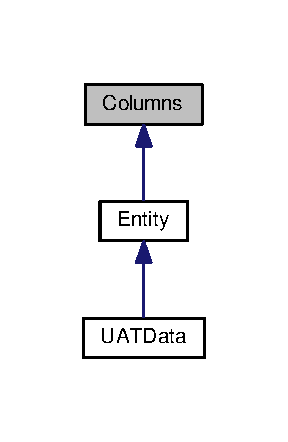
\includegraphics[width=138pt]{classColumns__inherit__graph}
\end{center}
\end{figure}
\subsection*{Public Member Functions}
\begin{DoxyCompactItemize}
\item 
bool \mbox{\hyperlink{classColumns_a4467704e26d0899a5873df4a28978cd2}{get}} (const char $\ast$key, int \&ref\+Var)
\item 
bool \mbox{\hyperlink{classColumns_acc2d0655f5329b618cdb31c844214daa}{get}} (const char $\ast$key, float \&ref\+Var)
\item 
bool \mbox{\hyperlink{classColumns_a4cb8a06d153469b71aa4de37968d6277}{get}} (const char $\ast$key, string \&ref\+Var)
\item 
bool \mbox{\hyperlink{classColumns_adf2ef04de02351dcbb3ab7e1fed5a7fe}{get}} (const char $\ast$key, bool \&ref\+Var)
\item 
void \mbox{\hyperlink{classColumns_a878cae2a1f8d3ee9e3b3f8dfae5a4a10}{set}} (const char $\ast$key, const int \&value)
\item 
void \mbox{\hyperlink{classColumns_a2c67a52aadc3501d509ff03a4990cada}{set}} (const char $\ast$key, const float \&value)
\item 
void \mbox{\hyperlink{classColumns_a1c0dc9986943b8152fa80dd53277fbd0}{set}} (const char $\ast$key, const string \&value)
\item 
void \mbox{\hyperlink{classColumns_a5eb2a1336790ed61ff1593561ebf6736}{set}} (const char $\ast$key, const bool \&value)
\item 
virtual \mbox{\hyperlink{datadefinition_8h_aec40b8d2d2c045d8af617ce94864651f}{schema}} \mbox{\hyperlink{classColumns_aeb2cbb10de5358d5c1f411f327324c94}{getschema}} () const
\item 
void \mbox{\hyperlink{classColumns_a47d00e2daee2c85a40952509a542a911}{clear}} ()
\end{DoxyCompactItemize}
\subsection*{Public Attributes}
\begin{DoxyCompactItemize}
\item 
\mbox{\hyperlink{datadefinition_8h_aea73dfd4c959e6737c9c65474e4529ec}{map\+Int}} \mbox{\hyperlink{classColumns_a8cbc620473c96a5e587fec5a7d7be695}{m\+\_\+int\+Columns}}
\item 
\mbox{\hyperlink{datadefinition_8h_a9ada3c20f161f474bb963207a7f7bde5}{map\+Str}} \mbox{\hyperlink{classColumns_a2a592e1dfc29b2daed0013d085854aa3}{m\+\_\+str\+Columns}}
\item 
\mbox{\hyperlink{datadefinition_8h_a143e5002d845b09ca5dcaf1eda71d70f}{map\+Bool}} \mbox{\hyperlink{classColumns_a454542a78d6dc1013881e2c3abdbd9f7}{m\+\_\+bool\+Columns}}
\item 
\mbox{\hyperlink{datadefinition_8h_aeaff661fb97ce7aa76f32e7e308f3a15}{map\+Float}} \mbox{\hyperlink{classColumns_ac0b423f0dcaa97fe42e2a0283c13d9bc}{m\+\_\+dbl\+Columns}}
\end{DoxyCompactItemize}


\subsection{Detailed Description}
This is a class that holds data for one row or one object at a time. It can hold data for only int, string, bool, float. But can be easily extended for more data types limited only by the ones supported by sqlite3. The specialized templated functions help seemlessly add values to the internal associative containers. 

\subsection{Member Function Documentation}
\mbox{\Hypertarget{classColumns_a47d00e2daee2c85a40952509a542a911}\label{classColumns_a47d00e2daee2c85a40952509a542a911}} 
\index{Columns@{Columns}!clear@{clear}}
\index{clear@{clear}!Columns@{Columns}}
\subsubsection{\texorpdfstring{clear()}{clear()}}
{\footnotesize\ttfamily void Columns\+::clear (\begin{DoxyParamCaption}{ }\end{DoxyParamCaption})\hspace{0.3cm}{\ttfamily [inline]}}

\mbox{\Hypertarget{classColumns_a4467704e26d0899a5873df4a28978cd2}\label{classColumns_a4467704e26d0899a5873df4a28978cd2}} 
\index{Columns@{Columns}!get@{get}}
\index{get@{get}!Columns@{Columns}}
\subsubsection{\texorpdfstring{get()}{get()}\hspace{0.1cm}{\footnotesize\ttfamily [1/4]}}
{\footnotesize\ttfamily bool Columns\+::get (\begin{DoxyParamCaption}\item[{const char $\ast$}]{key,  }\item[{int \&}]{ref\+Var }\end{DoxyParamCaption})}

\mbox{\Hypertarget{classColumns_acc2d0655f5329b618cdb31c844214daa}\label{classColumns_acc2d0655f5329b618cdb31c844214daa}} 
\index{Columns@{Columns}!get@{get}}
\index{get@{get}!Columns@{Columns}}
\subsubsection{\texorpdfstring{get()}{get()}\hspace{0.1cm}{\footnotesize\ttfamily [2/4]}}
{\footnotesize\ttfamily bool Columns\+::get (\begin{DoxyParamCaption}\item[{const char $\ast$}]{key,  }\item[{float \&}]{ref\+Var }\end{DoxyParamCaption})}

\mbox{\Hypertarget{classColumns_a4cb8a06d153469b71aa4de37968d6277}\label{classColumns_a4cb8a06d153469b71aa4de37968d6277}} 
\index{Columns@{Columns}!get@{get}}
\index{get@{get}!Columns@{Columns}}
\subsubsection{\texorpdfstring{get()}{get()}\hspace{0.1cm}{\footnotesize\ttfamily [3/4]}}
{\footnotesize\ttfamily bool Columns\+::get (\begin{DoxyParamCaption}\item[{const char $\ast$}]{key,  }\item[{string \&}]{ref\+Var }\end{DoxyParamCaption})}

\mbox{\Hypertarget{classColumns_adf2ef04de02351dcbb3ab7e1fed5a7fe}\label{classColumns_adf2ef04de02351dcbb3ab7e1fed5a7fe}} 
\index{Columns@{Columns}!get@{get}}
\index{get@{get}!Columns@{Columns}}
\subsubsection{\texorpdfstring{get()}{get()}\hspace{0.1cm}{\footnotesize\ttfamily [4/4]}}
{\footnotesize\ttfamily bool Columns\+::get (\begin{DoxyParamCaption}\item[{const char $\ast$}]{key,  }\item[{bool \&}]{ref\+Var }\end{DoxyParamCaption})}

\mbox{\Hypertarget{classColumns_aeb2cbb10de5358d5c1f411f327324c94}\label{classColumns_aeb2cbb10de5358d5c1f411f327324c94}} 
\index{Columns@{Columns}!getschema@{getschema}}
\index{getschema@{getschema}!Columns@{Columns}}
\subsubsection{\texorpdfstring{getschema()}{getschema()}}
{\footnotesize\ttfamily \mbox{\hyperlink{datadefinition_8h_aec40b8d2d2c045d8af617ce94864651f}{schema}} Columns\+::getschema (\begin{DoxyParamCaption}{ }\end{DoxyParamCaption}) const\hspace{0.3cm}{\ttfamily [virtual]}}



Reimplemented in \mbox{\hyperlink{classUATData_a33290ef354a04c15d5262ccc7500411b}{U\+A\+T\+Data}}.

\mbox{\Hypertarget{classColumns_a878cae2a1f8d3ee9e3b3f8dfae5a4a10}\label{classColumns_a878cae2a1f8d3ee9e3b3f8dfae5a4a10}} 
\index{Columns@{Columns}!set@{set}}
\index{set@{set}!Columns@{Columns}}
\subsubsection{\texorpdfstring{set()}{set()}\hspace{0.1cm}{\footnotesize\ttfamily [1/4]}}
{\footnotesize\ttfamily void Columns\+::set (\begin{DoxyParamCaption}\item[{const char $\ast$}]{key,  }\item[{const int \&}]{value }\end{DoxyParamCaption})}

\mbox{\Hypertarget{classColumns_a2c67a52aadc3501d509ff03a4990cada}\label{classColumns_a2c67a52aadc3501d509ff03a4990cada}} 
\index{Columns@{Columns}!set@{set}}
\index{set@{set}!Columns@{Columns}}
\subsubsection{\texorpdfstring{set()}{set()}\hspace{0.1cm}{\footnotesize\ttfamily [2/4]}}
{\footnotesize\ttfamily void Columns\+::set (\begin{DoxyParamCaption}\item[{const char $\ast$}]{key,  }\item[{const float \&}]{value }\end{DoxyParamCaption})}

\mbox{\Hypertarget{classColumns_a1c0dc9986943b8152fa80dd53277fbd0}\label{classColumns_a1c0dc9986943b8152fa80dd53277fbd0}} 
\index{Columns@{Columns}!set@{set}}
\index{set@{set}!Columns@{Columns}}
\subsubsection{\texorpdfstring{set()}{set()}\hspace{0.1cm}{\footnotesize\ttfamily [3/4]}}
{\footnotesize\ttfamily void Columns\+::set (\begin{DoxyParamCaption}\item[{const char $\ast$}]{key,  }\item[{const string \&}]{value }\end{DoxyParamCaption})}

\mbox{\Hypertarget{classColumns_a5eb2a1336790ed61ff1593561ebf6736}\label{classColumns_a5eb2a1336790ed61ff1593561ebf6736}} 
\index{Columns@{Columns}!set@{set}}
\index{set@{set}!Columns@{Columns}}
\subsubsection{\texorpdfstring{set()}{set()}\hspace{0.1cm}{\footnotesize\ttfamily [4/4]}}
{\footnotesize\ttfamily void Columns\+::set (\begin{DoxyParamCaption}\item[{const char $\ast$}]{key,  }\item[{const bool \&}]{value }\end{DoxyParamCaption})}



\subsection{Member Data Documentation}
\mbox{\Hypertarget{classColumns_a454542a78d6dc1013881e2c3abdbd9f7}\label{classColumns_a454542a78d6dc1013881e2c3abdbd9f7}} 
\index{Columns@{Columns}!m\+\_\+bool\+Columns@{m\+\_\+bool\+Columns}}
\index{m\+\_\+bool\+Columns@{m\+\_\+bool\+Columns}!Columns@{Columns}}
\subsubsection{\texorpdfstring{m\+\_\+bool\+Columns}{m\_boolColumns}}
{\footnotesize\ttfamily \mbox{\hyperlink{datadefinition_8h_a143e5002d845b09ca5dcaf1eda71d70f}{map\+Bool}} Columns\+::m\+\_\+bool\+Columns}

\mbox{\Hypertarget{classColumns_ac0b423f0dcaa97fe42e2a0283c13d9bc}\label{classColumns_ac0b423f0dcaa97fe42e2a0283c13d9bc}} 
\index{Columns@{Columns}!m\+\_\+dbl\+Columns@{m\+\_\+dbl\+Columns}}
\index{m\+\_\+dbl\+Columns@{m\+\_\+dbl\+Columns}!Columns@{Columns}}
\subsubsection{\texorpdfstring{m\+\_\+dbl\+Columns}{m\_dblColumns}}
{\footnotesize\ttfamily \mbox{\hyperlink{datadefinition_8h_aeaff661fb97ce7aa76f32e7e308f3a15}{map\+Float}} Columns\+::m\+\_\+dbl\+Columns}

\mbox{\Hypertarget{classColumns_a8cbc620473c96a5e587fec5a7d7be695}\label{classColumns_a8cbc620473c96a5e587fec5a7d7be695}} 
\index{Columns@{Columns}!m\+\_\+int\+Columns@{m\+\_\+int\+Columns}}
\index{m\+\_\+int\+Columns@{m\+\_\+int\+Columns}!Columns@{Columns}}
\subsubsection{\texorpdfstring{m\+\_\+int\+Columns}{m\_intColumns}}
{\footnotesize\ttfamily \mbox{\hyperlink{datadefinition_8h_aea73dfd4c959e6737c9c65474e4529ec}{map\+Int}} Columns\+::m\+\_\+int\+Columns}

\mbox{\Hypertarget{classColumns_a2a592e1dfc29b2daed0013d085854aa3}\label{classColumns_a2a592e1dfc29b2daed0013d085854aa3}} 
\index{Columns@{Columns}!m\+\_\+str\+Columns@{m\+\_\+str\+Columns}}
\index{m\+\_\+str\+Columns@{m\+\_\+str\+Columns}!Columns@{Columns}}
\subsubsection{\texorpdfstring{m\+\_\+str\+Columns}{m\_strColumns}}
{\footnotesize\ttfamily \mbox{\hyperlink{datadefinition_8h_a9ada3c20f161f474bb963207a7f7bde5}{map\+Str}} Columns\+::m\+\_\+str\+Columns}



The documentation for this class was generated from the following files\+:\begin{DoxyCompactItemize}
\item 
sqlite-\/core/\+Headers/\mbox{\hyperlink{columns_8h}{columns.\+h}}\item 
sqlite-\/core/\+Sources/\mbox{\hyperlink{columns_8cpp}{columns.\+cpp}}\end{DoxyCompactItemize}

\hypertarget{classColumnsFromSqlValue}{}\section{Columns\+From\+Sql\+Value Class Reference}
\label{classColumnsFromSqlValue}\index{Columns\+From\+Sql\+Value@{Columns\+From\+Sql\+Value}}


{\ttfamily \#include \char`\"{}databroker.\+h\char`\"{}}

\subsection*{Static Public Member Functions}
\begin{DoxyCompactItemize}
\item 
static \mbox{\hyperlink{datadefinition_8h_a09c0cd32f8797a9ad3df7daa788656cc}{map\+Sql\+Value}} \mbox{\hyperlink{classColumnsFromSqlValue_a2bd2302c62e85d239d5d4debc92e5588}{map\+From\+Vec}} (const vector$<$ \mbox{\hyperlink{structSqlValue}{Sql\+Value}} $>$ \&values)
\item 
static \mbox{\hyperlink{classColumns}{Columns}} \mbox{\hyperlink{classColumnsFromSqlValue_ad6e30f90a769968da9e2de5181eeb8ca}{create}} (const \mbox{\hyperlink{datadefinition_8h_aec40b8d2d2c045d8af617ce94864651f}{schema}} \&\mbox{\hyperlink{datadefinition_8h_aec40b8d2d2c045d8af617ce94864651f}{schema}}, const vector$<$ \mbox{\hyperlink{structSqlValue}{Sql\+Value}} $>$ \&values)
\end{DoxyCompactItemize}


\subsection{Member Function Documentation}
\mbox{\Hypertarget{classColumnsFromSqlValue_ad6e30f90a769968da9e2de5181eeb8ca}\label{classColumnsFromSqlValue_ad6e30f90a769968da9e2de5181eeb8ca}} 
\index{Columns\+From\+Sql\+Value@{Columns\+From\+Sql\+Value}!create@{create}}
\index{create@{create}!Columns\+From\+Sql\+Value@{Columns\+From\+Sql\+Value}}
\subsubsection{\texorpdfstring{create()}{create()}}
{\footnotesize\ttfamily static \mbox{\hyperlink{classColumns}{Columns}} Columns\+From\+Sql\+Value\+::create (\begin{DoxyParamCaption}\item[{const \mbox{\hyperlink{datadefinition_8h_aec40b8d2d2c045d8af617ce94864651f}{schema}} \&}]{schema,  }\item[{const vector$<$ \mbox{\hyperlink{structSqlValue}{Sql\+Value}} $>$ \&}]{values }\end{DoxyParamCaption})\hspace{0.3cm}{\ttfamily [inline]}, {\ttfamily [static]}}

\mbox{\Hypertarget{classColumnsFromSqlValue_a2bd2302c62e85d239d5d4debc92e5588}\label{classColumnsFromSqlValue_a2bd2302c62e85d239d5d4debc92e5588}} 
\index{Columns\+From\+Sql\+Value@{Columns\+From\+Sql\+Value}!map\+From\+Vec@{map\+From\+Vec}}
\index{map\+From\+Vec@{map\+From\+Vec}!Columns\+From\+Sql\+Value@{Columns\+From\+Sql\+Value}}
\subsubsection{\texorpdfstring{map\+From\+Vec()}{mapFromVec()}}
{\footnotesize\ttfamily static \mbox{\hyperlink{datadefinition_8h_a09c0cd32f8797a9ad3df7daa788656cc}{map\+Sql\+Value}} Columns\+From\+Sql\+Value\+::map\+From\+Vec (\begin{DoxyParamCaption}\item[{const vector$<$ \mbox{\hyperlink{structSqlValue}{Sql\+Value}} $>$ \&}]{values }\end{DoxyParamCaption})\hspace{0.3cm}{\ttfamily [inline]}, {\ttfamily [static]}}



The documentation for this class was generated from the following file\+:\begin{DoxyCompactItemize}
\item 
sqlite-\/core/\+Headers/\mbox{\hyperlink{databroker_8h}{databroker.\+h}}\end{DoxyCompactItemize}

\hypertarget{classDB}{}\section{DB Class Reference}
\label{classDB}\index{DB@{DB}}


{\ttfamily \#include \char`\"{}db.\+h\char`\"{}}

\subsection*{Public Member Functions}
\begin{DoxyCompactItemize}
\item 
\mbox{\hyperlink{classDB_a1a7f3eafecf0e5834f03026c7f42e7ad}{DB}} (const char $\ast$name)
\item 
\mbox{\hyperlink{db_8h_a8c50929ef9b94683ef6653b885e5b9ed}{sqldb}} \mbox{\hyperlink{classDB_a669630d5015f0a02c649484feb228f57}{create}} () const
\item 
int \mbox{\hyperlink{classDB_aa81d5bd268236cb48a89717924c957d2}{exec\+Scalar}} (const char $\ast$sql) const
\item 
int \mbox{\hyperlink{classDB_a19e12469303264225f563b14c15bc2e6}{select\+Count\+Scalar}} (const char $\ast$sql) const
\item 
int \mbox{\hyperlink{classDB_a3b98437bd8c113a2bdd3a3bbbe499f85}{select\+Scalar}} (const char $\ast$sql, \mbox{\hyperlink{structSqlValue}{Sql\+Value}} \&sql\+Value) const
\item 
int \mbox{\hyperlink{classDB_a415cfd60411cfaaba4e88939a54e51eb}{select}} (const char $\ast$sql, \mbox{\hyperlink{db_8h_a356f4bbcc8528145c25584033ef0bcb8}{sql\+Result}} \&result) const
\end{DoxyCompactItemize}
\subsection*{Static Public Member Functions}
\begin{DoxyCompactItemize}
\item 
static int \mbox{\hyperlink{classDB_ac0dbe2bbb16c4519de0cc7754269abed}{callback}} (void $\ast$data, int argc, char $\ast$$\ast$argv, char $\ast$$\ast$az\+Col\+Name)
\end{DoxyCompactItemize}
\subsection*{Private Attributes}
\begin{DoxyCompactItemize}
\item 
const char $\ast$ \mbox{\hyperlink{classDB_a8ab4c5c7842069a778f6d4f14c15ed65}{m\+\_\+name}}
\end{DoxyCompactItemize}


\subsection{Detailed Description}
All database related operations are performed in this class only. 

\subsection{Constructor \& Destructor Documentation}
\mbox{\Hypertarget{classDB_a1a7f3eafecf0e5834f03026c7f42e7ad}\label{classDB_a1a7f3eafecf0e5834f03026c7f42e7ad}} 
\index{DB@{DB}!DB@{DB}}
\index{DB@{DB}!DB@{DB}}
\subsubsection{\texorpdfstring{D\+B()}{DB()}}
{\footnotesize\ttfamily D\+B\+::\+DB (\begin{DoxyParamCaption}\item[{const char $\ast$}]{name }\end{DoxyParamCaption})}



\subsection{Member Function Documentation}
\mbox{\Hypertarget{classDB_ac0dbe2bbb16c4519de0cc7754269abed}\label{classDB_ac0dbe2bbb16c4519de0cc7754269abed}} 
\index{DB@{DB}!callback@{callback}}
\index{callback@{callback}!DB@{DB}}
\subsubsection{\texorpdfstring{callback()}{callback()}}
{\footnotesize\ttfamily int D\+B\+::callback (\begin{DoxyParamCaption}\item[{void $\ast$}]{data,  }\item[{int}]{argc,  }\item[{char $\ast$$\ast$}]{argv,  }\item[{char $\ast$$\ast$}]{az\+Col\+Name }\end{DoxyParamCaption})\hspace{0.3cm}{\ttfamily [static]}}

\mbox{\Hypertarget{classDB_a669630d5015f0a02c649484feb228f57}\label{classDB_a669630d5015f0a02c649484feb228f57}} 
\index{DB@{DB}!create@{create}}
\index{create@{create}!DB@{DB}}
\subsubsection{\texorpdfstring{create()}{create()}}
{\footnotesize\ttfamily \mbox{\hyperlink{db_8h_a8c50929ef9b94683ef6653b885e5b9ed}{sqldb}} D\+B\+::create (\begin{DoxyParamCaption}{ }\end{DoxyParamCaption}) const}

The create function returns a sqlite3 db held in a unique\+\_\+ptr, ensuring safety from memory leakage. \mbox{\Hypertarget{classDB_aa81d5bd268236cb48a89717924c957d2}\label{classDB_aa81d5bd268236cb48a89717924c957d2}} 
\index{DB@{DB}!exec\+Scalar@{exec\+Scalar}}
\index{exec\+Scalar@{exec\+Scalar}!DB@{DB}}
\subsubsection{\texorpdfstring{exec\+Scalar()}{execScalar()}}
{\footnotesize\ttfamily int D\+B\+::exec\+Scalar (\begin{DoxyParamCaption}\item[{const char $\ast$}]{sql }\end{DoxyParamCaption}) const}

This function can be used for executing queries that are not run for any direct data. It can be used for Insert, Update, Delete. It returns if the operation executed successfully. \mbox{\Hypertarget{classDB_a415cfd60411cfaaba4e88939a54e51eb}\label{classDB_a415cfd60411cfaaba4e88939a54e51eb}} 
\index{DB@{DB}!select@{select}}
\index{select@{select}!DB@{DB}}
\subsubsection{\texorpdfstring{select()}{select()}}
{\footnotesize\ttfamily int D\+B\+::select (\begin{DoxyParamCaption}\item[{const char $\ast$}]{sql,  }\item[{\mbox{\hyperlink{db_8h_a356f4bbcc8528145c25584033ef0bcb8}{sql\+Result}} \&}]{result }\end{DoxyParamCaption}) const}

The function most helpful with select statements. It returns a vector of a vector of a \mbox{\hyperlink{structSqlValue}{Sql\+Value}} (representing one column). The return value returns the number of rows present in the table against the query. \mbox{\Hypertarget{classDB_a19e12469303264225f563b14c15bc2e6}\label{classDB_a19e12469303264225f563b14c15bc2e6}} 
\index{DB@{DB}!select\+Count\+Scalar@{select\+Count\+Scalar}}
\index{select\+Count\+Scalar@{select\+Count\+Scalar}!DB@{DB}}
\subsubsection{\texorpdfstring{select\+Count\+Scalar()}{selectCountScalar()}}
{\footnotesize\ttfamily int D\+B\+::select\+Count\+Scalar (\begin{DoxyParamCaption}\item[{const char $\ast$}]{sql }\end{DoxyParamCaption}) const}

The function can be used to find how many rows of data exist for a query or if a record exists in the table at all. It can be helpful for queries where we need to check if table exists. \mbox{\Hypertarget{classDB_a3b98437bd8c113a2bdd3a3bbbe499f85}\label{classDB_a3b98437bd8c113a2bdd3a3bbbe499f85}} 
\index{DB@{DB}!select\+Scalar@{select\+Scalar}}
\index{select\+Scalar@{select\+Scalar}!DB@{DB}}
\subsubsection{\texorpdfstring{select\+Scalar()}{selectScalar()}}
{\footnotesize\ttfamily int D\+B\+::select\+Scalar (\begin{DoxyParamCaption}\item[{const char $\ast$}]{sql,  }\item[{\mbox{\hyperlink{structSqlValue}{Sql\+Value}} \&}]{sql\+Value }\end{DoxyParamCaption}) const}

The function helps getting one single value from any one column or the first column depending on the query. 

\subsection{Member Data Documentation}
\mbox{\Hypertarget{classDB_a8ab4c5c7842069a778f6d4f14c15ed65}\label{classDB_a8ab4c5c7842069a778f6d4f14c15ed65}} 
\index{DB@{DB}!m\+\_\+name@{m\+\_\+name}}
\index{m\+\_\+name@{m\+\_\+name}!DB@{DB}}
\subsubsection{\texorpdfstring{m\+\_\+name}{m\_name}}
{\footnotesize\ttfamily const char$\ast$ D\+B\+::m\+\_\+name\hspace{0.3cm}{\ttfamily [private]}}



The documentation for this class was generated from the following files\+:\begin{DoxyCompactItemize}
\item 
sqlite-\/core/\+Headers/\mbox{\hyperlink{db_8h}{db.\+h}}\item 
sqlite-\/core/\+Sources/\mbox{\hyperlink{db_8cpp}{db.\+cpp}}\end{DoxyCompactItemize}

\hypertarget{classDbManager}{}\section{Db\+Manager$<$ Entity\+Creation\+Policy $>$ Class Template Reference}
\label{classDbManager}\index{Db\+Manager$<$ Entity\+Creation\+Policy $>$@{Db\+Manager$<$ Entity\+Creation\+Policy $>$}}


{\ttfamily \#include \char`\"{}dbmanager.\+h\char`\"{}}



Inheritance diagram for Db\+Manager$<$ Entity\+Creation\+Policy $>$\+:\nopagebreak
\begin{figure}[H]
\begin{center}
\leavevmode
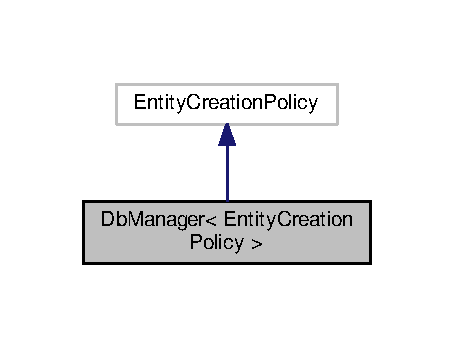
\includegraphics[width=218pt]{classDbManager__inherit__graph}
\end{center}
\end{figure}


Collaboration diagram for Db\+Manager$<$ Entity\+Creation\+Policy $>$\+:\nopagebreak
\begin{figure}[H]
\begin{center}
\leavevmode
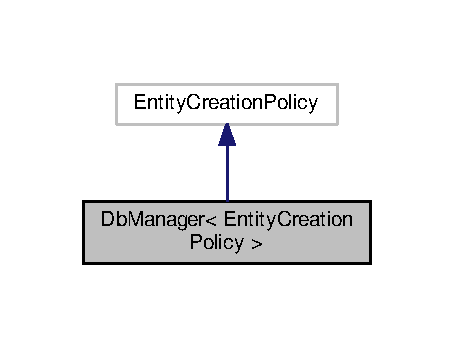
\includegraphics[width=218pt]{classDbManager__coll__graph}
\end{center}
\end{figure}
\subsection*{Static Public Member Functions}
\begin{DoxyCompactItemize}
\item 
static \mbox{\hyperlink{classDbManager}{Db\+Manager}} \mbox{\hyperlink{classDbManager_ab470cdc17355eec8153533c74d022298}{instance}} ()
\end{DoxyCompactItemize}
\subsection*{Protected Member Functions}
\begin{DoxyCompactItemize}
\item 
\mbox{\hyperlink{classDbManager_a303a0e1b940c528144c7a698943d4dae}{Db\+Manager}} ()=default
\end{DoxyCompactItemize}


\subsection{Detailed Description}
\subsubsection*{template$<$class Entity\+Creation\+Policy = Default\+Data\+Creation\+Policy$>$\newline
class Db\+Manager$<$ Entity\+Creation\+Policy $>$}

The class that creates recipe for an object according to the way it has to be created and then finally saved. This class shall hold more features in future that will help configure object creation, serialization and deserialization. 

\subsection{Constructor \& Destructor Documentation}
\mbox{\Hypertarget{classDbManager_a303a0e1b940c528144c7a698943d4dae}\label{classDbManager_a303a0e1b940c528144c7a698943d4dae}} 
\index{Db\+Manager@{Db\+Manager}!Db\+Manager@{Db\+Manager}}
\index{Db\+Manager@{Db\+Manager}!Db\+Manager@{Db\+Manager}}
\subsubsection{\texorpdfstring{Db\+Manager()}{DbManager()}}
{\footnotesize\ttfamily template$<$class Entity\+Creation\+Policy  = Default\+Data\+Creation\+Policy$>$ \\
\mbox{\hyperlink{classDbManager}{Db\+Manager}}$<$ Entity\+Creation\+Policy $>$\+::\mbox{\hyperlink{classDbManager}{Db\+Manager}} (\begin{DoxyParamCaption}{ }\end{DoxyParamCaption})\hspace{0.3cm}{\ttfamily [protected]}, {\ttfamily [default]}}



\subsection{Member Function Documentation}
\mbox{\Hypertarget{classDbManager_ab470cdc17355eec8153533c74d022298}\label{classDbManager_ab470cdc17355eec8153533c74d022298}} 
\index{Db\+Manager@{Db\+Manager}!instance@{instance}}
\index{instance@{instance}!Db\+Manager@{Db\+Manager}}
\subsubsection{\texorpdfstring{instance()}{instance()}}
{\footnotesize\ttfamily template$<$class Entity\+Creation\+Policy  = Default\+Data\+Creation\+Policy$>$ \\
static \mbox{\hyperlink{classDbManager}{Db\+Manager}} \mbox{\hyperlink{classDbManager}{Db\+Manager}}$<$ Entity\+Creation\+Policy $>$\+::instance (\begin{DoxyParamCaption}{ }\end{DoxyParamCaption})\hspace{0.3cm}{\ttfamily [inline]}, {\ttfamily [static]}}



The documentation for this class was generated from the following file\+:\begin{DoxyCompactItemize}
\item 
sqlite-\/core/\+Headers/\mbox{\hyperlink{dbmanager_8h}{dbmanager.\+h}}\end{DoxyCompactItemize}

\hypertarget{classDefaultDataCreationPolicy}{}\section{Default\+Data\+Creation\+Policy Class Reference}
\label{classDefaultDataCreationPolicy}\index{Default\+Data\+Creation\+Policy@{Default\+Data\+Creation\+Policy}}


{\ttfamily \#include \char`\"{}dbmanager.\+h\char`\"{}}

\subsection*{Public Member Functions}
\begin{DoxyCompactItemize}
\item 
{\footnotesize template$<$class Any\+Data\+Type $>$ }\\Any\+Data\+Type \mbox{\hyperlink{classDefaultDataCreationPolicy_a6ac123fffc1c6210dea6709cf4a76c3b}{Create}} (const char $\ast$db\+Name, const char $\ast$table\+Name)
\end{DoxyCompactItemize}


\subsection{Member Function Documentation}
\mbox{\Hypertarget{classDefaultDataCreationPolicy_a6ac123fffc1c6210dea6709cf4a76c3b}\label{classDefaultDataCreationPolicy_a6ac123fffc1c6210dea6709cf4a76c3b}} 
\index{Default\+Data\+Creation\+Policy@{Default\+Data\+Creation\+Policy}!Create@{Create}}
\index{Create@{Create}!Default\+Data\+Creation\+Policy@{Default\+Data\+Creation\+Policy}}
\subsubsection{\texorpdfstring{Create()}{Create()}}
{\footnotesize\ttfamily template$<$class Any\+Data\+Type $>$ \\
Any\+Data\+Type Default\+Data\+Creation\+Policy\+::\+Create (\begin{DoxyParamCaption}\item[{const char $\ast$}]{db\+Name,  }\item[{const char $\ast$}]{table\+Name }\end{DoxyParamCaption})\hspace{0.3cm}{\ttfamily [inline]}}



The documentation for this class was generated from the following file\+:\begin{DoxyCompactItemize}
\item 
sqlite-\/core/\+Headers/\mbox{\hyperlink{dbmanager_8h}{dbmanager.\+h}}\end{DoxyCompactItemize}

\hypertarget{classEntity}{}\section{Entity Class Reference}
\label{classEntity}\index{Entity@{Entity}}


{\ttfamily \#include \char`\"{}entity.\+h\char`\"{}}



Inheritance diagram for Entity\+:\nopagebreak
\begin{figure}[H]
\begin{center}
\leavevmode
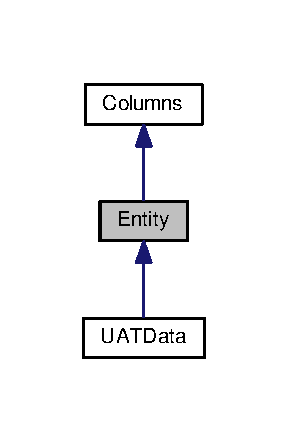
\includegraphics[width=138pt]{classEntity__inherit__graph}
\end{center}
\end{figure}


Collaboration diagram for Entity\+:\nopagebreak
\begin{figure}[H]
\begin{center}
\leavevmode
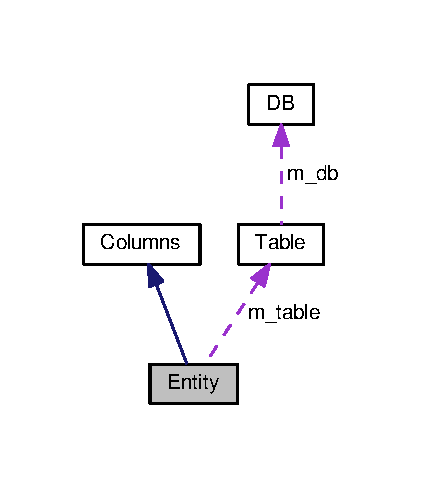
\includegraphics[width=203pt]{classEntity__coll__graph}
\end{center}
\end{figure}
\subsection*{Public Member Functions}
\begin{DoxyCompactItemize}
\item 
\mbox{\hyperlink{classEntity_a123f776b73726fba47ee376b2f903ea7}{Entity}} (const char $\ast$db\+Name, const char $\ast$table\+Name)
\item 
void \mbox{\hyperlink{classEntity_adb45cf2a74f4ce58b340b70e1727c8e5}{Save}} ()
\item 
virtual void \mbox{\hyperlink{classEntity_a0f8088e06ee1aae86e0a8049e371692f}{set\+Data}} ()
\end{DoxyCompactItemize}
\subsection*{Protected Member Functions}
\begin{DoxyCompactItemize}
\item 
\mbox{\hyperlink{classColumns}{Columns}} \mbox{\hyperlink{classEntity_a3b769f023811c9f6d8b6d18305173703}{first}} ()
\item 
\mbox{\hyperlink{classColumns}{Columns}} \mbox{\hyperlink{classEntity_a55872541f5b73a8cef49eda0368c770c}{last}} ()
\item 
std\+::vector$<$ \mbox{\hyperlink{classColumns}{Columns}} $>$ \mbox{\hyperlink{classEntity_aae8be1f7e39217b5abf629e5149958c5}{all}} ()
\end{DoxyCompactItemize}
\subsection*{Private Attributes}
\begin{DoxyCompactItemize}
\item 
\mbox{\hyperlink{classTable}{Table}} \mbox{\hyperlink{classEntity_a7492e529485203a402122b8f3e09dfb6}{m\+\_\+table}}
\end{DoxyCompactItemize}
\subsection*{Additional Inherited Members}


\subsection{Detailed Description}
The bae class for any data type that we want to save to database. The class can be decomposed further to derive policies related to saving data and then initializing user defined data objects from basic types. 

\subsection{Constructor \& Destructor Documentation}
\mbox{\Hypertarget{classEntity_a123f776b73726fba47ee376b2f903ea7}\label{classEntity_a123f776b73726fba47ee376b2f903ea7}} 
\index{Entity@{Entity}!Entity@{Entity}}
\index{Entity@{Entity}!Entity@{Entity}}
\subsubsection{\texorpdfstring{Entity()}{Entity()}}
{\footnotesize\ttfamily Entity\+::\+Entity (\begin{DoxyParamCaption}\item[{const char $\ast$}]{db\+Name,  }\item[{const char $\ast$}]{table\+Name }\end{DoxyParamCaption})\hspace{0.3cm}{\ttfamily [inline]}}



\subsection{Member Function Documentation}
\mbox{\Hypertarget{classEntity_aae8be1f7e39217b5abf629e5149958c5}\label{classEntity_aae8be1f7e39217b5abf629e5149958c5}} 
\index{Entity@{Entity}!all@{all}}
\index{all@{all}!Entity@{Entity}}
\subsubsection{\texorpdfstring{all()}{all()}}
{\footnotesize\ttfamily std\+::vector$<$\mbox{\hyperlink{classColumns}{Columns}}$>$ Entity\+::all (\begin{DoxyParamCaption}{ }\end{DoxyParamCaption})\hspace{0.3cm}{\ttfamily [inline]}, {\ttfamily [protected]}}

\mbox{\Hypertarget{classEntity_a3b769f023811c9f6d8b6d18305173703}\label{classEntity_a3b769f023811c9f6d8b6d18305173703}} 
\index{Entity@{Entity}!first@{first}}
\index{first@{first}!Entity@{Entity}}
\subsubsection{\texorpdfstring{first()}{first()}}
{\footnotesize\ttfamily \mbox{\hyperlink{classColumns}{Columns}} Entity\+::first (\begin{DoxyParamCaption}{ }\end{DoxyParamCaption})\hspace{0.3cm}{\ttfamily [inline]}, {\ttfamily [protected]}}

A helper function that returns first value from db \mbox{\Hypertarget{classEntity_a55872541f5b73a8cef49eda0368c770c}\label{classEntity_a55872541f5b73a8cef49eda0368c770c}} 
\index{Entity@{Entity}!last@{last}}
\index{last@{last}!Entity@{Entity}}
\subsubsection{\texorpdfstring{last()}{last()}}
{\footnotesize\ttfamily \mbox{\hyperlink{classColumns}{Columns}} Entity\+::last (\begin{DoxyParamCaption}{ }\end{DoxyParamCaption})\hspace{0.3cm}{\ttfamily [inline]}, {\ttfamily [protected]}}

\mbox{\Hypertarget{classEntity_adb45cf2a74f4ce58b340b70e1727c8e5}\label{classEntity_adb45cf2a74f4ce58b340b70e1727c8e5}} 
\index{Entity@{Entity}!Save@{Save}}
\index{Save@{Save}!Entity@{Entity}}
\subsubsection{\texorpdfstring{Save()}{Save()}}
{\footnotesize\ttfamily void Entity\+::\+Save (\begin{DoxyParamCaption}{ }\end{DoxyParamCaption})\hspace{0.3cm}{\ttfamily [inline]}}

\mbox{\Hypertarget{classEntity_a0f8088e06ee1aae86e0a8049e371692f}\label{classEntity_a0f8088e06ee1aae86e0a8049e371692f}} 
\index{Entity@{Entity}!set\+Data@{set\+Data}}
\index{set\+Data@{set\+Data}!Entity@{Entity}}
\subsubsection{\texorpdfstring{set\+Data()}{setData()}}
{\footnotesize\ttfamily virtual void Entity\+::set\+Data (\begin{DoxyParamCaption}{ }\end{DoxyParamCaption})\hspace{0.3cm}{\ttfamily [inline]}, {\ttfamily [virtual]}}



Reimplemented in \mbox{\hyperlink{classUATData_a969aa1661ec27cd3b85999fc61403a0e}{U\+A\+T\+Data}}.



\subsection{Member Data Documentation}
\mbox{\Hypertarget{classEntity_a7492e529485203a402122b8f3e09dfb6}\label{classEntity_a7492e529485203a402122b8f3e09dfb6}} 
\index{Entity@{Entity}!m\+\_\+table@{m\+\_\+table}}
\index{m\+\_\+table@{m\+\_\+table}!Entity@{Entity}}
\subsubsection{\texorpdfstring{m\+\_\+table}{m\_table}}
{\footnotesize\ttfamily \mbox{\hyperlink{classTable}{Table}} Entity\+::m\+\_\+table\hspace{0.3cm}{\ttfamily [private]}}



The documentation for this class was generated from the following file\+:\begin{DoxyCompactItemize}
\item 
sqlite-\/core/\+Headers/\mbox{\hyperlink{entity_8h}{entity.\+h}}\end{DoxyCompactItemize}

\hypertarget{classSqlFactory}{}\section{Sql\+Factory Class Reference}
\label{classSqlFactory}\index{Sql\+Factory@{Sql\+Factory}}


{\ttfamily \#include \char`\"{}sqlfactory.\+h\char`\"{}}

\subsection*{Static Public Member Functions}
\begin{DoxyCompactItemize}
\item 
static std\+::string \mbox{\hyperlink{classSqlFactory_a46f4bbef3a8868e711ac6a832cc4fee3}{treat\+Sql\+Value}} (string value, \mbox{\hyperlink{datadefinition_8h_ad06ef517a8bb3398f146f81f18988b9f}{Sql\+Type\+Enum}} type)
\item 
static string \mbox{\hyperlink{classSqlFactory_a3dcc73772b677e2e739e7130c9886615}{T\+A\+B\+L\+E\+\_\+\+E\+X\+I\+S\+TS}} (const char $\ast$tablename)
\item 
static std\+::string \mbox{\hyperlink{classSqlFactory_a0500a06f7e113a0921eec11e2d39ce80}{C\+R\+E\+A\+T\+E\+\_\+\+T\+A\+B\+LE}} (const char $\ast$table\+Name, vector$<$ \mbox{\hyperlink{structSqlField}{Sql\+Field}} $>$ sql\+Fields)
\item 
static std\+::string \mbox{\hyperlink{classSqlFactory_a9819d8d4683d97617ec2a9dcd5c462a4}{I\+N\+S\+E\+R\+T\+\_\+\+T\+A\+B\+LE}} (const char $\ast$table\+Name, std\+::string names, std\+::string values)
\item 
static std\+::string \mbox{\hyperlink{classSqlFactory_aa3bf3f1cf57e9980d740809a249db516}{I\+N\+S\+E\+R\+T\+\_\+\+T\+A\+B\+LE}} (const char $\ast$table\+Name, vector$<$ string $>$ names, vector$<$ string $>$ values)
\item 
static std\+::string \mbox{\hyperlink{classSqlFactory_a40368c3142309ffaec984147fd6ebad5}{S\+E\+L\+E\+CT}} (const char $\ast$table\+Name, int count)
\end{DoxyCompactItemize}
\subsection*{Static Private Member Functions}
\begin{DoxyCompactItemize}
\item 
static void \mbox{\hyperlink{classSqlFactory_a1ce0da51370f2723f3ca34f40c3ae9ea}{join}} (const vector$<$ string $>$ \&v, char c, string \&s)
\item 
static const char $\ast$ \mbox{\hyperlink{classSqlFactory_a760a8ef85d6503d858b174363c909f00}{Sql\+Type\+Enum\+\_\+\+To\+\_\+\+Str}} (\mbox{\hyperlink{datadefinition_8h_ad06ef517a8bb3398f146f81f18988b9f}{Sql\+Type\+Enum}} type)
\item 
static std\+::string \mbox{\hyperlink{classSqlFactory_a4bf8f30773341eba53e287bd6c2ef4c6}{field\+Specs}} (\mbox{\hyperlink{datadefinition_8h_ad06ef517a8bb3398f146f81f18988b9f}{Sql\+Type\+Enum}} type, int sz=0, bool is\+Key=false, bool not\+Null=false)
\item 
static std\+::string \mbox{\hyperlink{classSqlFactory_a28ad43892f8c9c7b207d8dced28e2ae2}{ddl\+Cat}} (\mbox{\hyperlink{structSqlField}{Sql\+Field}} field)
\end{DoxyCompactItemize}


\subsection{Detailed Description}
This is the class where all sql strings are made out of the data that it receives from client objects. It has functions for I\+N\+S\+E\+RT, S\+E\+L\+E\+CT and C\+R\+E\+A\+TE T\+A\+B\+LE. More can be added in due course. 

\subsection{Member Function Documentation}
\mbox{\Hypertarget{classSqlFactory_a0500a06f7e113a0921eec11e2d39ce80}\label{classSqlFactory_a0500a06f7e113a0921eec11e2d39ce80}} 
\index{Sql\+Factory@{Sql\+Factory}!C\+R\+E\+A\+T\+E\+\_\+\+T\+A\+B\+LE@{C\+R\+E\+A\+T\+E\+\_\+\+T\+A\+B\+LE}}
\index{C\+R\+E\+A\+T\+E\+\_\+\+T\+A\+B\+LE@{C\+R\+E\+A\+T\+E\+\_\+\+T\+A\+B\+LE}!Sql\+Factory@{Sql\+Factory}}
\subsubsection{\texorpdfstring{C\+R\+E\+A\+T\+E\+\_\+\+T\+A\+B\+L\+E()}{CREATE\_TABLE()}}
{\footnotesize\ttfamily static std\+::string Sql\+Factory\+::\+C\+R\+E\+A\+T\+E\+\_\+\+T\+A\+B\+LE (\begin{DoxyParamCaption}\item[{const char $\ast$}]{table\+Name,  }\item[{vector$<$ \mbox{\hyperlink{structSqlField}{Sql\+Field}} $>$}]{sql\+Fields }\end{DoxyParamCaption})\hspace{0.3cm}{\ttfamily [inline]}, {\ttfamily [static]}}

\mbox{\Hypertarget{classSqlFactory_a28ad43892f8c9c7b207d8dced28e2ae2}\label{classSqlFactory_a28ad43892f8c9c7b207d8dced28e2ae2}} 
\index{Sql\+Factory@{Sql\+Factory}!ddl\+Cat@{ddl\+Cat}}
\index{ddl\+Cat@{ddl\+Cat}!Sql\+Factory@{Sql\+Factory}}
\subsubsection{\texorpdfstring{ddl\+Cat()}{ddlCat()}}
{\footnotesize\ttfamily static std\+::string Sql\+Factory\+::ddl\+Cat (\begin{DoxyParamCaption}\item[{\mbox{\hyperlink{structSqlField}{Sql\+Field}}}]{field }\end{DoxyParamCaption})\hspace{0.3cm}{\ttfamily [inline]}, {\ttfamily [static]}, {\ttfamily [private]}}

\mbox{\Hypertarget{classSqlFactory_a4bf8f30773341eba53e287bd6c2ef4c6}\label{classSqlFactory_a4bf8f30773341eba53e287bd6c2ef4c6}} 
\index{Sql\+Factory@{Sql\+Factory}!field\+Specs@{field\+Specs}}
\index{field\+Specs@{field\+Specs}!Sql\+Factory@{Sql\+Factory}}
\subsubsection{\texorpdfstring{field\+Specs()}{fieldSpecs()}}
{\footnotesize\ttfamily static std\+::string Sql\+Factory\+::field\+Specs (\begin{DoxyParamCaption}\item[{\mbox{\hyperlink{datadefinition_8h_ad06ef517a8bb3398f146f81f18988b9f}{Sql\+Type\+Enum}}}]{type,  }\item[{int}]{sz = {\ttfamily 0},  }\item[{bool}]{is\+Key = {\ttfamily false},  }\item[{bool}]{not\+Null = {\ttfamily false} }\end{DoxyParamCaption})\hspace{0.3cm}{\ttfamily [inline]}, {\ttfamily [static]}, {\ttfamily [private]}}

\mbox{\Hypertarget{classSqlFactory_a9819d8d4683d97617ec2a9dcd5c462a4}\label{classSqlFactory_a9819d8d4683d97617ec2a9dcd5c462a4}} 
\index{Sql\+Factory@{Sql\+Factory}!I\+N\+S\+E\+R\+T\+\_\+\+T\+A\+B\+LE@{I\+N\+S\+E\+R\+T\+\_\+\+T\+A\+B\+LE}}
\index{I\+N\+S\+E\+R\+T\+\_\+\+T\+A\+B\+LE@{I\+N\+S\+E\+R\+T\+\_\+\+T\+A\+B\+LE}!Sql\+Factory@{Sql\+Factory}}
\subsubsection{\texorpdfstring{I\+N\+S\+E\+R\+T\+\_\+\+T\+A\+B\+L\+E()}{INSERT\_TABLE()}\hspace{0.1cm}{\footnotesize\ttfamily [1/2]}}
{\footnotesize\ttfamily static std\+::string Sql\+Factory\+::\+I\+N\+S\+E\+R\+T\+\_\+\+T\+A\+B\+LE (\begin{DoxyParamCaption}\item[{const char $\ast$}]{table\+Name,  }\item[{std\+::string}]{names,  }\item[{std\+::string}]{values }\end{DoxyParamCaption})\hspace{0.3cm}{\ttfamily [inline]}, {\ttfamily [static]}}

\mbox{\Hypertarget{classSqlFactory_aa3bf3f1cf57e9980d740809a249db516}\label{classSqlFactory_aa3bf3f1cf57e9980d740809a249db516}} 
\index{Sql\+Factory@{Sql\+Factory}!I\+N\+S\+E\+R\+T\+\_\+\+T\+A\+B\+LE@{I\+N\+S\+E\+R\+T\+\_\+\+T\+A\+B\+LE}}
\index{I\+N\+S\+E\+R\+T\+\_\+\+T\+A\+B\+LE@{I\+N\+S\+E\+R\+T\+\_\+\+T\+A\+B\+LE}!Sql\+Factory@{Sql\+Factory}}
\subsubsection{\texorpdfstring{I\+N\+S\+E\+R\+T\+\_\+\+T\+A\+B\+L\+E()}{INSERT\_TABLE()}\hspace{0.1cm}{\footnotesize\ttfamily [2/2]}}
{\footnotesize\ttfamily static std\+::string Sql\+Factory\+::\+I\+N\+S\+E\+R\+T\+\_\+\+T\+A\+B\+LE (\begin{DoxyParamCaption}\item[{const char $\ast$}]{table\+Name,  }\item[{vector$<$ string $>$}]{names,  }\item[{vector$<$ string $>$}]{values }\end{DoxyParamCaption})\hspace{0.3cm}{\ttfamily [inline]}, {\ttfamily [static]}}

\mbox{\Hypertarget{classSqlFactory_a1ce0da51370f2723f3ca34f40c3ae9ea}\label{classSqlFactory_a1ce0da51370f2723f3ca34f40c3ae9ea}} 
\index{Sql\+Factory@{Sql\+Factory}!join@{join}}
\index{join@{join}!Sql\+Factory@{Sql\+Factory}}
\subsubsection{\texorpdfstring{join()}{join()}}
{\footnotesize\ttfamily static void Sql\+Factory\+::join (\begin{DoxyParamCaption}\item[{const vector$<$ string $>$ \&}]{v,  }\item[{char}]{c,  }\item[{string \&}]{s }\end{DoxyParamCaption})\hspace{0.3cm}{\ttfamily [inline]}, {\ttfamily [static]}, {\ttfamily [private]}}

\mbox{\Hypertarget{classSqlFactory_a40368c3142309ffaec984147fd6ebad5}\label{classSqlFactory_a40368c3142309ffaec984147fd6ebad5}} 
\index{Sql\+Factory@{Sql\+Factory}!S\+E\+L\+E\+CT@{S\+E\+L\+E\+CT}}
\index{S\+E\+L\+E\+CT@{S\+E\+L\+E\+CT}!Sql\+Factory@{Sql\+Factory}}
\subsubsection{\texorpdfstring{S\+E\+L\+E\+C\+T()}{SELECT()}}
{\footnotesize\ttfamily static std\+::string Sql\+Factory\+::\+S\+E\+L\+E\+CT (\begin{DoxyParamCaption}\item[{const char $\ast$}]{table\+Name,  }\item[{int}]{count }\end{DoxyParamCaption})\hspace{0.3cm}{\ttfamily [inline]}, {\ttfamily [static]}}

\mbox{\Hypertarget{classSqlFactory_a760a8ef85d6503d858b174363c909f00}\label{classSqlFactory_a760a8ef85d6503d858b174363c909f00}} 
\index{Sql\+Factory@{Sql\+Factory}!Sql\+Type\+Enum\+\_\+\+To\+\_\+\+Str@{Sql\+Type\+Enum\+\_\+\+To\+\_\+\+Str}}
\index{Sql\+Type\+Enum\+\_\+\+To\+\_\+\+Str@{Sql\+Type\+Enum\+\_\+\+To\+\_\+\+Str}!Sql\+Factory@{Sql\+Factory}}
\subsubsection{\texorpdfstring{Sql\+Type\+Enum\+\_\+\+To\+\_\+\+Str()}{SqlTypeEnum\_To\_Str()}}
{\footnotesize\ttfamily static const char$\ast$ Sql\+Factory\+::\+Sql\+Type\+Enum\+\_\+\+To\+\_\+\+Str (\begin{DoxyParamCaption}\item[{\mbox{\hyperlink{datadefinition_8h_ad06ef517a8bb3398f146f81f18988b9f}{Sql\+Type\+Enum}}}]{type }\end{DoxyParamCaption})\hspace{0.3cm}{\ttfamily [inline]}, {\ttfamily [static]}, {\ttfamily [private]}}

\mbox{\Hypertarget{classSqlFactory_a3dcc73772b677e2e739e7130c9886615}\label{classSqlFactory_a3dcc73772b677e2e739e7130c9886615}} 
\index{Sql\+Factory@{Sql\+Factory}!T\+A\+B\+L\+E\+\_\+\+E\+X\+I\+S\+TS@{T\+A\+B\+L\+E\+\_\+\+E\+X\+I\+S\+TS}}
\index{T\+A\+B\+L\+E\+\_\+\+E\+X\+I\+S\+TS@{T\+A\+B\+L\+E\+\_\+\+E\+X\+I\+S\+TS}!Sql\+Factory@{Sql\+Factory}}
\subsubsection{\texorpdfstring{T\+A\+B\+L\+E\+\_\+\+E\+X\+I\+S\+T\+S()}{TABLE\_EXISTS()}}
{\footnotesize\ttfamily static string Sql\+Factory\+::\+T\+A\+B\+L\+E\+\_\+\+E\+X\+I\+S\+TS (\begin{DoxyParamCaption}\item[{const char $\ast$}]{tablename }\end{DoxyParamCaption})\hspace{0.3cm}{\ttfamily [inline]}, {\ttfamily [static]}}

\mbox{\Hypertarget{classSqlFactory_a46f4bbef3a8868e711ac6a832cc4fee3}\label{classSqlFactory_a46f4bbef3a8868e711ac6a832cc4fee3}} 
\index{Sql\+Factory@{Sql\+Factory}!treat\+Sql\+Value@{treat\+Sql\+Value}}
\index{treat\+Sql\+Value@{treat\+Sql\+Value}!Sql\+Factory@{Sql\+Factory}}
\subsubsection{\texorpdfstring{treat\+Sql\+Value()}{treatSqlValue()}}
{\footnotesize\ttfamily static std\+::string Sql\+Factory\+::treat\+Sql\+Value (\begin{DoxyParamCaption}\item[{string}]{value,  }\item[{\mbox{\hyperlink{datadefinition_8h_ad06ef517a8bb3398f146f81f18988b9f}{Sql\+Type\+Enum}}}]{type }\end{DoxyParamCaption})\hspace{0.3cm}{\ttfamily [inline]}, {\ttfamily [static]}}



The documentation for this class was generated from the following file\+:\begin{DoxyCompactItemize}
\item 
sqlite-\/core/\+Headers/\mbox{\hyperlink{sqlfactory_8h}{sqlfactory.\+h}}\end{DoxyCompactItemize}

\hypertarget{structSqlField}{}\section{Sql\+Field Struct Reference}
\label{structSqlField}\index{Sql\+Field@{Sql\+Field}}


{\ttfamily \#include \char`\"{}datadefinition.\+h\char`\"{}}

\subsection*{Public Member Functions}
\begin{DoxyCompactItemize}
\item 
\mbox{\hyperlink{structSqlField_af348c54a252bf9ae67e7f280737aa5d0}{Sql\+Field}} (const char $\ast$name, const \mbox{\hyperlink{datadefinition_8h_ad06ef517a8bb3398f146f81f18988b9f}{Sql\+Type\+Enum}} \&type=\mbox{\hyperlink{datadefinition_8h_ad06ef517a8bb3398f146f81f18988b9faa5ec7b1f6f558b362f5a9ced5f228c2b}{Sql\+Type\+Enum\+::\+S\+Q\+L\+\_\+\+S\+TR}}, const int \&sz=0, const bool \&is\+Key=false, const bool \&not\+Null=false)
\end{DoxyCompactItemize}
\subsection*{Static Public Member Functions}
\begin{DoxyCompactItemize}
\item 
static vector$<$ \mbox{\hyperlink{structSqlField}{Sql\+Field}} $>$ \mbox{\hyperlink{structSqlField_a4349ebac0f3a6ddbbd81fdb3fbc268f0}{from\+Sql\+Values}} (const vector$<$ \mbox{\hyperlink{structSqlValue}{Sql\+Value}} $>$ \&sql\+Values)
\end{DoxyCompactItemize}
\subsection*{Public Attributes}
\begin{DoxyCompactItemize}
\item 
const char $\ast$ \mbox{\hyperlink{structSqlField_ace03689493f338658646e0ac61d3a885}{Name}}
\item 
\mbox{\hyperlink{datadefinition_8h_ad06ef517a8bb3398f146f81f18988b9f}{Sql\+Type\+Enum}} \mbox{\hyperlink{structSqlField_afb3221f041d06f2c792e0eef1195d0cf}{Type}}
\item 
int \mbox{\hyperlink{structSqlField_aef1c65782455a79a4797ed16bf7f296b}{Sz}}
\item 
bool \mbox{\hyperlink{structSqlField_a21d13bd62ab5c18b750f050c449a0c2e}{Is\+Key}}
\item 
bool \mbox{\hyperlink{structSqlField_aed207960cbeff50c17adc5a11f94b4a9}{Not\+Null}}
\end{DoxyCompactItemize}


\subsection{Constructor \& Destructor Documentation}
\mbox{\Hypertarget{structSqlField_af348c54a252bf9ae67e7f280737aa5d0}\label{structSqlField_af348c54a252bf9ae67e7f280737aa5d0}} 
\index{Sql\+Field@{Sql\+Field}!Sql\+Field@{Sql\+Field}}
\index{Sql\+Field@{Sql\+Field}!Sql\+Field@{Sql\+Field}}
\subsubsection{\texorpdfstring{Sql\+Field()}{SqlField()}}
{\footnotesize\ttfamily Sql\+Field\+::\+Sql\+Field (\begin{DoxyParamCaption}\item[{const char $\ast$}]{name,  }\item[{const \mbox{\hyperlink{datadefinition_8h_ad06ef517a8bb3398f146f81f18988b9f}{Sql\+Type\+Enum}} \&}]{type = {\ttfamily \mbox{\hyperlink{datadefinition_8h_ad06ef517a8bb3398f146f81f18988b9faa5ec7b1f6f558b362f5a9ced5f228c2b}{Sql\+Type\+Enum\+::\+S\+Q\+L\+\_\+\+S\+TR}}},  }\item[{const int \&}]{sz = {\ttfamily 0},  }\item[{const bool \&}]{is\+Key = {\ttfamily false},  }\item[{const bool \&}]{not\+Null = {\ttfamily false} }\end{DoxyParamCaption})\hspace{0.3cm}{\ttfamily [inline]}}



\subsection{Member Function Documentation}
\mbox{\Hypertarget{structSqlField_a4349ebac0f3a6ddbbd81fdb3fbc268f0}\label{structSqlField_a4349ebac0f3a6ddbbd81fdb3fbc268f0}} 
\index{Sql\+Field@{Sql\+Field}!from\+Sql\+Values@{from\+Sql\+Values}}
\index{from\+Sql\+Values@{from\+Sql\+Values}!Sql\+Field@{Sql\+Field}}
\subsubsection{\texorpdfstring{from\+Sql\+Values()}{fromSqlValues()}}
{\footnotesize\ttfamily static vector$<$\mbox{\hyperlink{structSqlField}{Sql\+Field}}$>$ Sql\+Field\+::from\+Sql\+Values (\begin{DoxyParamCaption}\item[{const vector$<$ \mbox{\hyperlink{structSqlValue}{Sql\+Value}} $>$ \&}]{sql\+Values }\end{DoxyParamCaption})\hspace{0.3cm}{\ttfamily [inline]}, {\ttfamily [static]}}



\subsection{Member Data Documentation}
\mbox{\Hypertarget{structSqlField_a21d13bd62ab5c18b750f050c449a0c2e}\label{structSqlField_a21d13bd62ab5c18b750f050c449a0c2e}} 
\index{Sql\+Field@{Sql\+Field}!Is\+Key@{Is\+Key}}
\index{Is\+Key@{Is\+Key}!Sql\+Field@{Sql\+Field}}
\subsubsection{\texorpdfstring{Is\+Key}{IsKey}}
{\footnotesize\ttfamily bool Sql\+Field\+::\+Is\+Key}

\mbox{\Hypertarget{structSqlField_ace03689493f338658646e0ac61d3a885}\label{structSqlField_ace03689493f338658646e0ac61d3a885}} 
\index{Sql\+Field@{Sql\+Field}!Name@{Name}}
\index{Name@{Name}!Sql\+Field@{Sql\+Field}}
\subsubsection{\texorpdfstring{Name}{Name}}
{\footnotesize\ttfamily const char$\ast$ Sql\+Field\+::\+Name}

\mbox{\Hypertarget{structSqlField_aed207960cbeff50c17adc5a11f94b4a9}\label{structSqlField_aed207960cbeff50c17adc5a11f94b4a9}} 
\index{Sql\+Field@{Sql\+Field}!Not\+Null@{Not\+Null}}
\index{Not\+Null@{Not\+Null}!Sql\+Field@{Sql\+Field}}
\subsubsection{\texorpdfstring{Not\+Null}{NotNull}}
{\footnotesize\ttfamily bool Sql\+Field\+::\+Not\+Null}

\mbox{\Hypertarget{structSqlField_aef1c65782455a79a4797ed16bf7f296b}\label{structSqlField_aef1c65782455a79a4797ed16bf7f296b}} 
\index{Sql\+Field@{Sql\+Field}!Sz@{Sz}}
\index{Sz@{Sz}!Sql\+Field@{Sql\+Field}}
\subsubsection{\texorpdfstring{Sz}{Sz}}
{\footnotesize\ttfamily int Sql\+Field\+::\+Sz}

\mbox{\Hypertarget{structSqlField_afb3221f041d06f2c792e0eef1195d0cf}\label{structSqlField_afb3221f041d06f2c792e0eef1195d0cf}} 
\index{Sql\+Field@{Sql\+Field}!Type@{Type}}
\index{Type@{Type}!Sql\+Field@{Sql\+Field}}
\subsubsection{\texorpdfstring{Type}{Type}}
{\footnotesize\ttfamily \mbox{\hyperlink{datadefinition_8h_ad06ef517a8bb3398f146f81f18988b9f}{Sql\+Type\+Enum}} Sql\+Field\+::\+Type}



The documentation for this struct was generated from the following file\+:\begin{DoxyCompactItemize}
\item 
sqlite-\/core/\+Headers/\mbox{\hyperlink{datadefinition_8h}{datadefinition.\+h}}\end{DoxyCompactItemize}

\hypertarget{structsqlite3__deleter}{}\section{sqlite3\+\_\+deleter Struct Reference}
\label{structsqlite3__deleter}\index{sqlite3\+\_\+deleter@{sqlite3\+\_\+deleter}}


{\ttfamily \#include \char`\"{}db.\+h\char`\"{}}

\subsection*{Public Member Functions}
\begin{DoxyCompactItemize}
\item 
void \mbox{\hyperlink{structsqlite3__deleter_a03feba9176a8e2e0c02d56ec8314018b}{operator()}} (sqlite3 $\ast$db)
\end{DoxyCompactItemize}


\subsection{Member Function Documentation}
\mbox{\Hypertarget{structsqlite3__deleter_a03feba9176a8e2e0c02d56ec8314018b}\label{structsqlite3__deleter_a03feba9176a8e2e0c02d56ec8314018b}} 
\index{sqlite3\+\_\+deleter@{sqlite3\+\_\+deleter}!operator()@{operator()}}
\index{operator()@{operator()}!sqlite3\+\_\+deleter@{sqlite3\+\_\+deleter}}
\subsubsection{\texorpdfstring{operator()()}{operator()()}}
{\footnotesize\ttfamily void sqlite3\+\_\+deleter\+::operator() (\begin{DoxyParamCaption}\item[{sqlite3 $\ast$}]{db }\end{DoxyParamCaption})\hspace{0.3cm}{\ttfamily [inline]}}



The documentation for this struct was generated from the following file\+:\begin{DoxyCompactItemize}
\item 
sqlite-\/core/\+Headers/\mbox{\hyperlink{db_8h}{db.\+h}}\end{DoxyCompactItemize}

\hypertarget{structsqlite3__stmt__deleter}{}\section{sqlite3\+\_\+stmt\+\_\+deleter Struct Reference}
\label{structsqlite3__stmt__deleter}\index{sqlite3\+\_\+stmt\+\_\+deleter@{sqlite3\+\_\+stmt\+\_\+deleter}}


{\ttfamily \#include \char`\"{}db.\+h\char`\"{}}

\subsection*{Public Member Functions}
\begin{DoxyCompactItemize}
\item 
void \mbox{\hyperlink{structsqlite3__stmt__deleter_a0d25181a866b19111f63cce0fce0c789}{operator()}} (sqlite3\+\_\+stmt $\ast$stmt)
\end{DoxyCompactItemize}


\subsection{Member Function Documentation}
\mbox{\Hypertarget{structsqlite3__stmt__deleter_a0d25181a866b19111f63cce0fce0c789}\label{structsqlite3__stmt__deleter_a0d25181a866b19111f63cce0fce0c789}} 
\index{sqlite3\+\_\+stmt\+\_\+deleter@{sqlite3\+\_\+stmt\+\_\+deleter}!operator()@{operator()}}
\index{operator()@{operator()}!sqlite3\+\_\+stmt\+\_\+deleter@{sqlite3\+\_\+stmt\+\_\+deleter}}
\subsubsection{\texorpdfstring{operator()()}{operator()()}}
{\footnotesize\ttfamily void sqlite3\+\_\+stmt\+\_\+deleter\+::operator() (\begin{DoxyParamCaption}\item[{sqlite3\+\_\+stmt $\ast$}]{stmt }\end{DoxyParamCaption})\hspace{0.3cm}{\ttfamily [inline]}}



The documentation for this struct was generated from the following file\+:\begin{DoxyCompactItemize}
\item 
sqlite-\/core/\+Headers/\mbox{\hyperlink{db_8h}{db.\+h}}\end{DoxyCompactItemize}

\hypertarget{structSqlValue}{}\section{Sql\+Value Struct Reference}
\label{structSqlValue}\index{Sql\+Value@{Sql\+Value}}


{\ttfamily \#include \char`\"{}datadefinition.\+h\char`\"{}}

\subsection*{Public Member Functions}
\begin{DoxyCompactItemize}
\item 
\mbox{\hyperlink{structSqlValue_a35ecbd8591181b12dbbc954046a6380a}{Sql\+Value}} ()=default
\item 
\mbox{\hyperlink{structSqlValue_ad1e1270b387de26ffdabb4a702304446}{Sql\+Value}} (const char $\ast$name, const int \&int\+Val)
\item 
\mbox{\hyperlink{structSqlValue_a434e7637b0a06e43c2d1b84556470f53}{Sql\+Value}} (const char $\ast$name, const string \&char\+Val)
\item 
\mbox{\hyperlink{structSqlValue_aaa5d565de799694e1f1ed216251b3eee}{Sql\+Value}} (const char $\ast$name, const float \&dbl\+Val)
\item 
\mbox{\hyperlink{structSqlValue_ad93f72e6c40c913a16dfa39573912f2b}{Sql\+Value}} (const char $\ast$name)
\item 
string \mbox{\hyperlink{structSqlValue_a0daacca986ce795c69c8022651fe5873}{to\+String}} ()
\end{DoxyCompactItemize}
\subsection*{Public Attributes}
\begin{DoxyCompactItemize}
\item 
\mbox{\hyperlink{datadefinition_8h_ad06ef517a8bb3398f146f81f18988b9f}{Sql\+Type\+Enum}} \mbox{\hyperlink{structSqlValue_a59eef92117d6b8685a8970cad60c340e}{Tp}}
\item 
int \mbox{\hyperlink{structSqlValue_a237610d8d49573b3351c494c87cb0f7f}{Int\+Val}} = 0
\item 
string \mbox{\hyperlink{structSqlValue_ad867a5a62a7935a8106945672a1928c9}{Txt\+Val}} = \char`\"{}\char`\"{}
\item 
float \mbox{\hyperlink{structSqlValue_a542ff56bf66bba588e89f72de93eaf5a}{Flt\+Val}} = 0
\item 
const char $\ast$ \mbox{\hyperlink{structSqlValue_a160fa9b84cdf9bf9dc452392570d6a11}{Name}}
\end{DoxyCompactItemize}


\subsection{Detailed Description}
This stucture holds value of one column coming from the sqlite3 db. They can be any type. While initializing the object, it is determined as to what data type the column is initialized as. This struct can be improved in many ways. To begin with, it could be converted into a union. 

\subsection{Constructor \& Destructor Documentation}
\mbox{\Hypertarget{structSqlValue_a35ecbd8591181b12dbbc954046a6380a}\label{structSqlValue_a35ecbd8591181b12dbbc954046a6380a}} 
\index{Sql\+Value@{Sql\+Value}!Sql\+Value@{Sql\+Value}}
\index{Sql\+Value@{Sql\+Value}!Sql\+Value@{Sql\+Value}}
\subsubsection{\texorpdfstring{Sql\+Value()}{SqlValue()}\hspace{0.1cm}{\footnotesize\ttfamily [1/5]}}
{\footnotesize\ttfamily Sql\+Value\+::\+Sql\+Value (\begin{DoxyParamCaption}{ }\end{DoxyParamCaption})\hspace{0.3cm}{\ttfamily [default]}}

\mbox{\Hypertarget{structSqlValue_ad1e1270b387de26ffdabb4a702304446}\label{structSqlValue_ad1e1270b387de26ffdabb4a702304446}} 
\index{Sql\+Value@{Sql\+Value}!Sql\+Value@{Sql\+Value}}
\index{Sql\+Value@{Sql\+Value}!Sql\+Value@{Sql\+Value}}
\subsubsection{\texorpdfstring{Sql\+Value()}{SqlValue()}\hspace{0.1cm}{\footnotesize\ttfamily [2/5]}}
{\footnotesize\ttfamily Sql\+Value\+::\+Sql\+Value (\begin{DoxyParamCaption}\item[{const char $\ast$}]{name,  }\item[{const int \&}]{int\+Val }\end{DoxyParamCaption})\hspace{0.3cm}{\ttfamily [inline]}}

\mbox{\Hypertarget{structSqlValue_a434e7637b0a06e43c2d1b84556470f53}\label{structSqlValue_a434e7637b0a06e43c2d1b84556470f53}} 
\index{Sql\+Value@{Sql\+Value}!Sql\+Value@{Sql\+Value}}
\index{Sql\+Value@{Sql\+Value}!Sql\+Value@{Sql\+Value}}
\subsubsection{\texorpdfstring{Sql\+Value()}{SqlValue()}\hspace{0.1cm}{\footnotesize\ttfamily [3/5]}}
{\footnotesize\ttfamily Sql\+Value\+::\+Sql\+Value (\begin{DoxyParamCaption}\item[{const char $\ast$}]{name,  }\item[{const string \&}]{char\+Val }\end{DoxyParamCaption})\hspace{0.3cm}{\ttfamily [inline]}}

\mbox{\Hypertarget{structSqlValue_aaa5d565de799694e1f1ed216251b3eee}\label{structSqlValue_aaa5d565de799694e1f1ed216251b3eee}} 
\index{Sql\+Value@{Sql\+Value}!Sql\+Value@{Sql\+Value}}
\index{Sql\+Value@{Sql\+Value}!Sql\+Value@{Sql\+Value}}
\subsubsection{\texorpdfstring{Sql\+Value()}{SqlValue()}\hspace{0.1cm}{\footnotesize\ttfamily [4/5]}}
{\footnotesize\ttfamily Sql\+Value\+::\+Sql\+Value (\begin{DoxyParamCaption}\item[{const char $\ast$}]{name,  }\item[{const float \&}]{dbl\+Val }\end{DoxyParamCaption})\hspace{0.3cm}{\ttfamily [inline]}}

\mbox{\Hypertarget{structSqlValue_ad93f72e6c40c913a16dfa39573912f2b}\label{structSqlValue_ad93f72e6c40c913a16dfa39573912f2b}} 
\index{Sql\+Value@{Sql\+Value}!Sql\+Value@{Sql\+Value}}
\index{Sql\+Value@{Sql\+Value}!Sql\+Value@{Sql\+Value}}
\subsubsection{\texorpdfstring{Sql\+Value()}{SqlValue()}\hspace{0.1cm}{\footnotesize\ttfamily [5/5]}}
{\footnotesize\ttfamily Sql\+Value\+::\+Sql\+Value (\begin{DoxyParamCaption}\item[{const char $\ast$}]{name }\end{DoxyParamCaption})\hspace{0.3cm}{\ttfamily [inline]}}



\subsection{Member Function Documentation}
\mbox{\Hypertarget{structSqlValue_a0daacca986ce795c69c8022651fe5873}\label{structSqlValue_a0daacca986ce795c69c8022651fe5873}} 
\index{Sql\+Value@{Sql\+Value}!to\+String@{to\+String}}
\index{to\+String@{to\+String}!Sql\+Value@{Sql\+Value}}
\subsubsection{\texorpdfstring{to\+String()}{toString()}}
{\footnotesize\ttfamily string Sql\+Value\+::to\+String (\begin{DoxyParamCaption}{ }\end{DoxyParamCaption})\hspace{0.3cm}{\ttfamily [inline]}}



\subsection{Member Data Documentation}
\mbox{\Hypertarget{structSqlValue_a542ff56bf66bba588e89f72de93eaf5a}\label{structSqlValue_a542ff56bf66bba588e89f72de93eaf5a}} 
\index{Sql\+Value@{Sql\+Value}!Flt\+Val@{Flt\+Val}}
\index{Flt\+Val@{Flt\+Val}!Sql\+Value@{Sql\+Value}}
\subsubsection{\texorpdfstring{Flt\+Val}{FltVal}}
{\footnotesize\ttfamily float Sql\+Value\+::\+Flt\+Val = 0}

\mbox{\Hypertarget{structSqlValue_a237610d8d49573b3351c494c87cb0f7f}\label{structSqlValue_a237610d8d49573b3351c494c87cb0f7f}} 
\index{Sql\+Value@{Sql\+Value}!Int\+Val@{Int\+Val}}
\index{Int\+Val@{Int\+Val}!Sql\+Value@{Sql\+Value}}
\subsubsection{\texorpdfstring{Int\+Val}{IntVal}}
{\footnotesize\ttfamily int Sql\+Value\+::\+Int\+Val = 0}

\mbox{\Hypertarget{structSqlValue_a160fa9b84cdf9bf9dc452392570d6a11}\label{structSqlValue_a160fa9b84cdf9bf9dc452392570d6a11}} 
\index{Sql\+Value@{Sql\+Value}!Name@{Name}}
\index{Name@{Name}!Sql\+Value@{Sql\+Value}}
\subsubsection{\texorpdfstring{Name}{Name}}
{\footnotesize\ttfamily const char$\ast$ Sql\+Value\+::\+Name}

\mbox{\Hypertarget{structSqlValue_a59eef92117d6b8685a8970cad60c340e}\label{structSqlValue_a59eef92117d6b8685a8970cad60c340e}} 
\index{Sql\+Value@{Sql\+Value}!Tp@{Tp}}
\index{Tp@{Tp}!Sql\+Value@{Sql\+Value}}
\subsubsection{\texorpdfstring{Tp}{Tp}}
{\footnotesize\ttfamily \mbox{\hyperlink{datadefinition_8h_ad06ef517a8bb3398f146f81f18988b9f}{Sql\+Type\+Enum}} Sql\+Value\+::\+Tp}

\mbox{\Hypertarget{structSqlValue_ad867a5a62a7935a8106945672a1928c9}\label{structSqlValue_ad867a5a62a7935a8106945672a1928c9}} 
\index{Sql\+Value@{Sql\+Value}!Txt\+Val@{Txt\+Val}}
\index{Txt\+Val@{Txt\+Val}!Sql\+Value@{Sql\+Value}}
\subsubsection{\texorpdfstring{Txt\+Val}{TxtVal}}
{\footnotesize\ttfamily string Sql\+Value\+::\+Txt\+Val = \char`\"{}\char`\"{}}



The documentation for this struct was generated from the following file\+:\begin{DoxyCompactItemize}
\item 
sqlite-\/core/\+Headers/\mbox{\hyperlink{datadefinition_8h}{datadefinition.\+h}}\end{DoxyCompactItemize}

\hypertarget{classSqlValueFromColumn}{}\section{Sql\+Value\+From\+Column Class Reference}
\label{classSqlValueFromColumn}\index{Sql\+Value\+From\+Column@{Sql\+Value\+From\+Column}}


{\ttfamily \#include \char`\"{}databroker.\+h\char`\"{}}

\subsection*{Static Public Member Functions}
\begin{DoxyCompactItemize}
\item 
static vector$<$ \mbox{\hyperlink{structSqlValue}{Sql\+Value}} $>$ \mbox{\hyperlink{classSqlValueFromColumn_a6e5d90bf8021211958258d2ea5e9c3a2}{create}} (\mbox{\hyperlink{classColumns}{Columns}} \&cols)
\end{DoxyCompactItemize}


\subsection{Member Function Documentation}
\mbox{\Hypertarget{classSqlValueFromColumn_a6e5d90bf8021211958258d2ea5e9c3a2}\label{classSqlValueFromColumn_a6e5d90bf8021211958258d2ea5e9c3a2}} 
\index{Sql\+Value\+From\+Column@{Sql\+Value\+From\+Column}!create@{create}}
\index{create@{create}!Sql\+Value\+From\+Column@{Sql\+Value\+From\+Column}}
\subsubsection{\texorpdfstring{create()}{create()}}
{\footnotesize\ttfamily static vector$<$\mbox{\hyperlink{structSqlValue}{Sql\+Value}}$>$ Sql\+Value\+From\+Column\+::create (\begin{DoxyParamCaption}\item[{\mbox{\hyperlink{classColumns}{Columns}} \&}]{cols }\end{DoxyParamCaption})\hspace{0.3cm}{\ttfamily [inline]}, {\ttfamily [static]}}



The documentation for this class was generated from the following file\+:\begin{DoxyCompactItemize}
\item 
sqlite-\/core/\+Headers/\mbox{\hyperlink{databroker_8h}{databroker.\+h}}\end{DoxyCompactItemize}

\hypertarget{classTable}{}\section{Table Class Reference}
\label{classTable}\index{Table@{Table}}


{\ttfamily \#include \char`\"{}table.\+h\char`\"{}}



Collaboration diagram for Table\+:\nopagebreak
\begin{figure}[H]
\begin{center}
\leavevmode
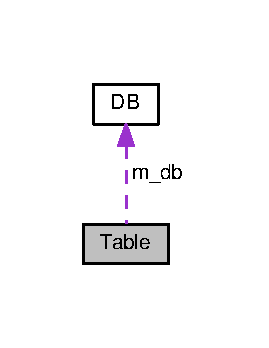
\includegraphics[width=129pt]{classTable__coll__graph}
\end{center}
\end{figure}
\subsection*{Public Member Functions}
\begin{DoxyCompactItemize}
\item 
\mbox{\hyperlink{classTable_ae35623804222a53627bdcaa9e180640f}{Table}} (const char $\ast$table\+Name, const char $\ast$db\+Name)
\item 
bool \mbox{\hyperlink{classTable_a46bf355769e7691ce79ff4363010dc7e}{istable\+Touched}} () const
\item 
bool \mbox{\hyperlink{classTable_a965f8ad5d716320501d64a121429ce50}{exists}} () const
\item 
void \mbox{\hyperlink{classTable_a861e8d9af1231690429629471fdd652b}{create}} (const vector$<$ \mbox{\hyperlink{structSqlField}{Sql\+Field}} $>$ \&fields)
\item 
void \mbox{\hyperlink{classTable_a4b2f3b62906af3f7548fc1ebd648dfc5}{save}} (const vector$<$ \mbox{\hyperlink{structSqlValue}{Sql\+Value}} $>$ \&values)
\item 
int \mbox{\hyperlink{classTable_af1ce76323b4045b893deaf05f51abfd0}{get}} (\mbox{\hyperlink{db_8h_a356f4bbcc8528145c25584033ef0bcb8}{sql\+Result}} \&results, int limit=0) const
\end{DoxyCompactItemize}
\subsection*{Private Attributes}
\begin{DoxyCompactItemize}
\item 
const char $\ast$ \mbox{\hyperlink{classTable_aaa150472b3686c7d86a5af58e7970f4a}{m\+\_\+name}}
\item 
\mbox{\hyperlink{classDB}{DB}} \mbox{\hyperlink{classTable_ab6a536f7b7619cd252c6f7b67909a505}{m\+\_\+db}}
\item 
bool \mbox{\hyperlink{classTable_a76e6e836dd4e86fa85064ed8a5f0d425}{m\+\_\+table\+Touched}}
\end{DoxyCompactItemize}


\subsection{Detailed Description}
This class is a broker between the front end classes and the \mbox{\hyperlink{classDB}{DB}} class that handles core db operations. This class gets data from fron-\/end classes, formats them using \mbox{\hyperlink{classSqlFactory}{Sql\+Factory}} class and passes them to the \mbox{\hyperlink{classDB}{DB}} class. 

\subsection{Constructor \& Destructor Documentation}
\mbox{\Hypertarget{classTable_ae35623804222a53627bdcaa9e180640f}\label{classTable_ae35623804222a53627bdcaa9e180640f}} 
\index{Table@{Table}!Table@{Table}}
\index{Table@{Table}!Table@{Table}}
\subsubsection{\texorpdfstring{Table()}{Table()}}
{\footnotesize\ttfamily Table\+::\+Table (\begin{DoxyParamCaption}\item[{const char $\ast$}]{table\+Name,  }\item[{const char $\ast$}]{db\+Name }\end{DoxyParamCaption})}



\subsection{Member Function Documentation}
\mbox{\Hypertarget{classTable_a861e8d9af1231690429629471fdd652b}\label{classTable_a861e8d9af1231690429629471fdd652b}} 
\index{Table@{Table}!create@{create}}
\index{create@{create}!Table@{Table}}
\subsubsection{\texorpdfstring{create()}{create()}}
{\footnotesize\ttfamily void Table\+::create (\begin{DoxyParamCaption}\item[{const vector$<$ \mbox{\hyperlink{structSqlField}{Sql\+Field}} $>$ \&}]{fields }\end{DoxyParamCaption})}

\mbox{\Hypertarget{classTable_a965f8ad5d716320501d64a121429ce50}\label{classTable_a965f8ad5d716320501d64a121429ce50}} 
\index{Table@{Table}!exists@{exists}}
\index{exists@{exists}!Table@{Table}}
\subsubsection{\texorpdfstring{exists()}{exists()}}
{\footnotesize\ttfamily bool Table\+::exists (\begin{DoxyParamCaption}{ }\end{DoxyParamCaption}) const}

\mbox{\Hypertarget{classTable_af1ce76323b4045b893deaf05f51abfd0}\label{classTable_af1ce76323b4045b893deaf05f51abfd0}} 
\index{Table@{Table}!get@{get}}
\index{get@{get}!Table@{Table}}
\subsubsection{\texorpdfstring{get()}{get()}}
{\footnotesize\ttfamily int Table\+::get (\begin{DoxyParamCaption}\item[{\mbox{\hyperlink{db_8h_a356f4bbcc8528145c25584033ef0bcb8}{sql\+Result}} \&}]{results,  }\item[{int}]{limit = {\ttfamily 0} }\end{DoxyParamCaption}) const}

\mbox{\Hypertarget{classTable_a46bf355769e7691ce79ff4363010dc7e}\label{classTable_a46bf355769e7691ce79ff4363010dc7e}} 
\index{Table@{Table}!istable\+Touched@{istable\+Touched}}
\index{istable\+Touched@{istable\+Touched}!Table@{Table}}
\subsubsection{\texorpdfstring{istable\+Touched()}{istableTouched()}}
{\footnotesize\ttfamily bool Table\+::istable\+Touched (\begin{DoxyParamCaption}{ }\end{DoxyParamCaption}) const\hspace{0.3cm}{\ttfamily [inline]}}

\mbox{\Hypertarget{classTable_a4b2f3b62906af3f7548fc1ebd648dfc5}\label{classTable_a4b2f3b62906af3f7548fc1ebd648dfc5}} 
\index{Table@{Table}!save@{save}}
\index{save@{save}!Table@{Table}}
\subsubsection{\texorpdfstring{save()}{save()}}
{\footnotesize\ttfamily void Table\+::save (\begin{DoxyParamCaption}\item[{const vector$<$ \mbox{\hyperlink{structSqlValue}{Sql\+Value}} $>$ \&}]{values }\end{DoxyParamCaption})}



\subsection{Member Data Documentation}
\mbox{\Hypertarget{classTable_ab6a536f7b7619cd252c6f7b67909a505}\label{classTable_ab6a536f7b7619cd252c6f7b67909a505}} 
\index{Table@{Table}!m\+\_\+db@{m\+\_\+db}}
\index{m\+\_\+db@{m\+\_\+db}!Table@{Table}}
\subsubsection{\texorpdfstring{m\+\_\+db}{m\_db}}
{\footnotesize\ttfamily \mbox{\hyperlink{classDB}{DB}} Table\+::m\+\_\+db\hspace{0.3cm}{\ttfamily [private]}}

\mbox{\Hypertarget{classTable_aaa150472b3686c7d86a5af58e7970f4a}\label{classTable_aaa150472b3686c7d86a5af58e7970f4a}} 
\index{Table@{Table}!m\+\_\+name@{m\+\_\+name}}
\index{m\+\_\+name@{m\+\_\+name}!Table@{Table}}
\subsubsection{\texorpdfstring{m\+\_\+name}{m\_name}}
{\footnotesize\ttfamily const char$\ast$ Table\+::m\+\_\+name\hspace{0.3cm}{\ttfamily [private]}}

\mbox{\Hypertarget{classTable_a76e6e836dd4e86fa85064ed8a5f0d425}\label{classTable_a76e6e836dd4e86fa85064ed8a5f0d425}} 
\index{Table@{Table}!m\+\_\+table\+Touched@{m\+\_\+table\+Touched}}
\index{m\+\_\+table\+Touched@{m\+\_\+table\+Touched}!Table@{Table}}
\subsubsection{\texorpdfstring{m\+\_\+table\+Touched}{m\_tableTouched}}
{\footnotesize\ttfamily bool Table\+::m\+\_\+table\+Touched\hspace{0.3cm}{\ttfamily [private]}}



The documentation for this class was generated from the following files\+:\begin{DoxyCompactItemize}
\item 
sqlite-\/core/\+Headers/\mbox{\hyperlink{table_8h}{table.\+h}}\item 
sqlite-\/core/\+Sources/\mbox{\hyperlink{table_8cpp}{table.\+cpp}}\end{DoxyCompactItemize}

\hypertarget{classUATData}{}\section{U\+A\+T\+Data Class Reference}
\label{classUATData}\index{U\+A\+T\+Data@{U\+A\+T\+Data}}


Inheritance diagram for U\+A\+T\+Data\+:\nopagebreak
\begin{figure}[H]
\begin{center}
\leavevmode
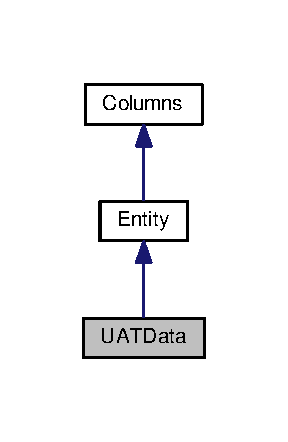
\includegraphics[width=138pt]{classUATData__inherit__graph}
\end{center}
\end{figure}


Collaboration diagram for U\+A\+T\+Data\+:\nopagebreak
\begin{figure}[H]
\begin{center}
\leavevmode
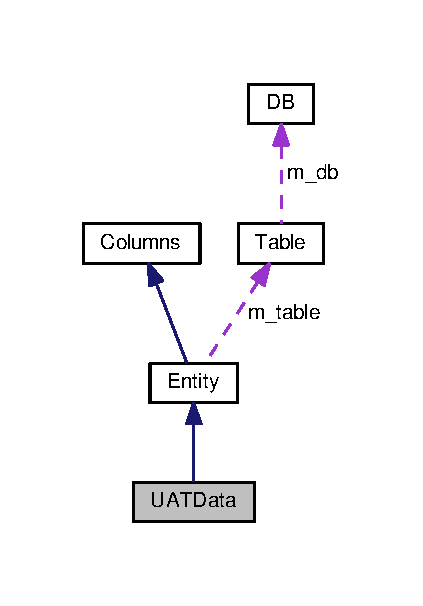
\includegraphics[width=203pt]{classUATData__coll__graph}
\end{center}
\end{figure}
\subsection*{Public Member Functions}
\begin{DoxyCompactItemize}
\item 
\mbox{\hyperlink{classUATData_a513b470878475946eca85bcb29810351}{U\+A\+T\+Data}} ()=default
\item 
\mbox{\hyperlink{classUATData_a5b4692dc1d8e0ad1a08358a4df27dc9d}{U\+A\+T\+Data}} (const char $\ast$db\+Name, const char $\ast$table\+Name)
\item 
void \mbox{\hyperlink{classUATData_a969aa1661ec27cd3b85999fc61403a0e}{set\+Data}} () override
\item 
\mbox{\hyperlink{datadefinition_8h_aec40b8d2d2c045d8af617ce94864651f}{schema}} \mbox{\hyperlink{classUATData_a33290ef354a04c15d5262ccc7500411b}{getschema}} () const override
\end{DoxyCompactItemize}
\subsection*{Public Attributes}
\begin{DoxyCompactItemize}
\item 
int \mbox{\hyperlink{classUATData_afa9b129b79280003eb7089447d77bf6d}{Latitude}}
\item 
int \mbox{\hyperlink{classUATData_a68f21f5af40cb1412ed4bc69a3e82305}{Longitude}}
\item 
bool \mbox{\hyperlink{classUATData_a8c2ca1eae7147dfdc99d2ea5b83a1763}{Air\+Ground\+State}}
\item 
float \mbox{\hyperlink{classUATData_a62c8c4089c4dc59347fca7cc569332b5}{Sig}}
\item 
string \mbox{\hyperlink{classUATData_ada1643b5e42b79e4a27bbf6d20505ef9}{N\+IC}}
\end{DoxyCompactItemize}
\subsection*{Additional Inherited Members}


\subsection{Detailed Description}
Test data, derives from Enity class to support core \mbox{\hyperlink{classDB}{DB}} features like save(), \mbox{\hyperlink{classColumns_a4467704e26d0899a5873df4a28978cd2}{get()}} 

\subsection{Constructor \& Destructor Documentation}
\mbox{\Hypertarget{classUATData_a513b470878475946eca85bcb29810351}\label{classUATData_a513b470878475946eca85bcb29810351}} 
\index{U\+A\+T\+Data@{U\+A\+T\+Data}!U\+A\+T\+Data@{U\+A\+T\+Data}}
\index{U\+A\+T\+Data@{U\+A\+T\+Data}!U\+A\+T\+Data@{U\+A\+T\+Data}}
\subsubsection{\texorpdfstring{U\+A\+T\+Data()}{UATData()}\hspace{0.1cm}{\footnotesize\ttfamily [1/2]}}
{\footnotesize\ttfamily U\+A\+T\+Data\+::\+U\+A\+T\+Data (\begin{DoxyParamCaption}{ }\end{DoxyParamCaption})\hspace{0.3cm}{\ttfamily [default]}}

\mbox{\Hypertarget{classUATData_a5b4692dc1d8e0ad1a08358a4df27dc9d}\label{classUATData_a5b4692dc1d8e0ad1a08358a4df27dc9d}} 
\index{U\+A\+T\+Data@{U\+A\+T\+Data}!U\+A\+T\+Data@{U\+A\+T\+Data}}
\index{U\+A\+T\+Data@{U\+A\+T\+Data}!U\+A\+T\+Data@{U\+A\+T\+Data}}
\subsubsection{\texorpdfstring{U\+A\+T\+Data()}{UATData()}\hspace{0.1cm}{\footnotesize\ttfamily [2/2]}}
{\footnotesize\ttfamily U\+A\+T\+Data\+::\+U\+A\+T\+Data (\begin{DoxyParamCaption}\item[{const char $\ast$}]{db\+Name,  }\item[{const char $\ast$}]{table\+Name }\end{DoxyParamCaption})\hspace{0.3cm}{\ttfamily [inline]}}



\subsection{Member Function Documentation}
\mbox{\Hypertarget{classUATData_a33290ef354a04c15d5262ccc7500411b}\label{classUATData_a33290ef354a04c15d5262ccc7500411b}} 
\index{U\+A\+T\+Data@{U\+A\+T\+Data}!getschema@{getschema}}
\index{getschema@{getschema}!U\+A\+T\+Data@{U\+A\+T\+Data}}
\subsubsection{\texorpdfstring{getschema()}{getschema()}}
{\footnotesize\ttfamily \mbox{\hyperlink{datadefinition_8h_aec40b8d2d2c045d8af617ce94864651f}{schema}} U\+A\+T\+Data\+::getschema (\begin{DoxyParamCaption}{ }\end{DoxyParamCaption}) const\hspace{0.3cm}{\ttfamily [inline]}, {\ttfamily [override]}, {\ttfamily [virtual]}}



Reimplemented from \mbox{\hyperlink{classColumns_aeb2cbb10de5358d5c1f411f327324c94}{Columns}}.

\mbox{\Hypertarget{classUATData_a969aa1661ec27cd3b85999fc61403a0e}\label{classUATData_a969aa1661ec27cd3b85999fc61403a0e}} 
\index{U\+A\+T\+Data@{U\+A\+T\+Data}!set\+Data@{set\+Data}}
\index{set\+Data@{set\+Data}!U\+A\+T\+Data@{U\+A\+T\+Data}}
\subsubsection{\texorpdfstring{set\+Data()}{setData()}}
{\footnotesize\ttfamily void U\+A\+T\+Data\+::set\+Data (\begin{DoxyParamCaption}{ }\end{DoxyParamCaption})\hspace{0.3cm}{\ttfamily [inline]}, {\ttfamily [override]}, {\ttfamily [virtual]}}

Overridden function, called internally when save is called on this entity object 

Reimplemented from \mbox{\hyperlink{classEntity_a0f8088e06ee1aae86e0a8049e371692f}{Entity}}.



\subsection{Member Data Documentation}
\mbox{\Hypertarget{classUATData_a8c2ca1eae7147dfdc99d2ea5b83a1763}\label{classUATData_a8c2ca1eae7147dfdc99d2ea5b83a1763}} 
\index{U\+A\+T\+Data@{U\+A\+T\+Data}!Air\+Ground\+State@{Air\+Ground\+State}}
\index{Air\+Ground\+State@{Air\+Ground\+State}!U\+A\+T\+Data@{U\+A\+T\+Data}}
\subsubsection{\texorpdfstring{Air\+Ground\+State}{AirGroundState}}
{\footnotesize\ttfamily bool U\+A\+T\+Data\+::\+Air\+Ground\+State}

\mbox{\Hypertarget{classUATData_afa9b129b79280003eb7089447d77bf6d}\label{classUATData_afa9b129b79280003eb7089447d77bf6d}} 
\index{U\+A\+T\+Data@{U\+A\+T\+Data}!Latitude@{Latitude}}
\index{Latitude@{Latitude}!U\+A\+T\+Data@{U\+A\+T\+Data}}
\subsubsection{\texorpdfstring{Latitude}{Latitude}}
{\footnotesize\ttfamily int U\+A\+T\+Data\+::\+Latitude}

\mbox{\Hypertarget{classUATData_a68f21f5af40cb1412ed4bc69a3e82305}\label{classUATData_a68f21f5af40cb1412ed4bc69a3e82305}} 
\index{U\+A\+T\+Data@{U\+A\+T\+Data}!Longitude@{Longitude}}
\index{Longitude@{Longitude}!U\+A\+T\+Data@{U\+A\+T\+Data}}
\subsubsection{\texorpdfstring{Longitude}{Longitude}}
{\footnotesize\ttfamily int U\+A\+T\+Data\+::\+Longitude}

\mbox{\Hypertarget{classUATData_ada1643b5e42b79e4a27bbf6d20505ef9}\label{classUATData_ada1643b5e42b79e4a27bbf6d20505ef9}} 
\index{U\+A\+T\+Data@{U\+A\+T\+Data}!N\+IC@{N\+IC}}
\index{N\+IC@{N\+IC}!U\+A\+T\+Data@{U\+A\+T\+Data}}
\subsubsection{\texorpdfstring{N\+IC}{NIC}}
{\footnotesize\ttfamily string U\+A\+T\+Data\+::\+N\+IC}

\mbox{\Hypertarget{classUATData_a62c8c4089c4dc59347fca7cc569332b5}\label{classUATData_a62c8c4089c4dc59347fca7cc569332b5}} 
\index{U\+A\+T\+Data@{U\+A\+T\+Data}!Sig@{Sig}}
\index{Sig@{Sig}!U\+A\+T\+Data@{U\+A\+T\+Data}}
\subsubsection{\texorpdfstring{Sig}{Sig}}
{\footnotesize\ttfamily float U\+A\+T\+Data\+::\+Sig}



The documentation for this class was generated from the following file\+:\begin{DoxyCompactItemize}
\item 
\mbox{\hyperlink{main_8cpp}{main.\+cpp}}\end{DoxyCompactItemize}

\hypertarget{classUATDomainCreationPolicy}{}\section{U\+A\+T\+Domain\+Creation\+Policy Class Reference}
\label{classUATDomainCreationPolicy}\index{U\+A\+T\+Domain\+Creation\+Policy@{U\+A\+T\+Domain\+Creation\+Policy}}
\subsection*{Public Member Functions}
\begin{DoxyCompactItemize}
\item 
{\footnotesize template$<$class U\+A\+T\+Data\+Type $>$ }\\U\+A\+T\+Data\+Type \mbox{\hyperlink{classUATDomainCreationPolicy_aced51b57b642cca926a77e90fbb7bfd3}{Create}} (const char $\ast$db\+Name, const char $\ast$table\+Name)
\end{DoxyCompactItemize}


\subsection{Detailed Description}
This is a data creation policy with a templated create function that creates the object for the type passed as an argument. A group of objects belonging to a specific domain (e.\+g. U\+AT) may follow a specific pattern when instantiated. A policy like this could be created for all such objects belonging to that group. 

\subsection{Member Function Documentation}
\mbox{\Hypertarget{classUATDomainCreationPolicy_aced51b57b642cca926a77e90fbb7bfd3}\label{classUATDomainCreationPolicy_aced51b57b642cca926a77e90fbb7bfd3}} 
\index{U\+A\+T\+Domain\+Creation\+Policy@{U\+A\+T\+Domain\+Creation\+Policy}!Create@{Create}}
\index{Create@{Create}!U\+A\+T\+Domain\+Creation\+Policy@{U\+A\+T\+Domain\+Creation\+Policy}}
\subsubsection{\texorpdfstring{Create()}{Create()}}
{\footnotesize\ttfamily template$<$class U\+A\+T\+Data\+Type $>$ \\
U\+A\+T\+Data\+Type U\+A\+T\+Domain\+Creation\+Policy\+::\+Create (\begin{DoxyParamCaption}\item[{const char $\ast$}]{db\+Name,  }\item[{const char $\ast$}]{table\+Name }\end{DoxyParamCaption})\hspace{0.3cm}{\ttfamily [inline]}}



The documentation for this class was generated from the following file\+:\begin{DoxyCompactItemize}
\item 
\mbox{\hyperlink{main_8cpp}{main.\+cpp}}\end{DoxyCompactItemize}

\chapter{File Documentation}
\hypertarget{main_8cpp}{}\section{main.\+cpp File Reference}
\label{main_8cpp}\index{main.\+cpp@{main.\+cpp}}
{\ttfamily \#include $<$iostream$>$}\newline
{\ttfamily \#include \char`\"{}dbmanager.\+h\char`\"{}}\newline
{\ttfamily \#include \char`\"{}db.\+h\char`\"{}}\newline
{\ttfamily \#include \char`\"{}table.\+h\char`\"{}}\newline
{\ttfamily \#include \char`\"{}entity.\+h\char`\"{}}\newline
Include dependency graph for main.\+cpp\+:\nopagebreak
\begin{figure}[H]
\begin{center}
\leavevmode
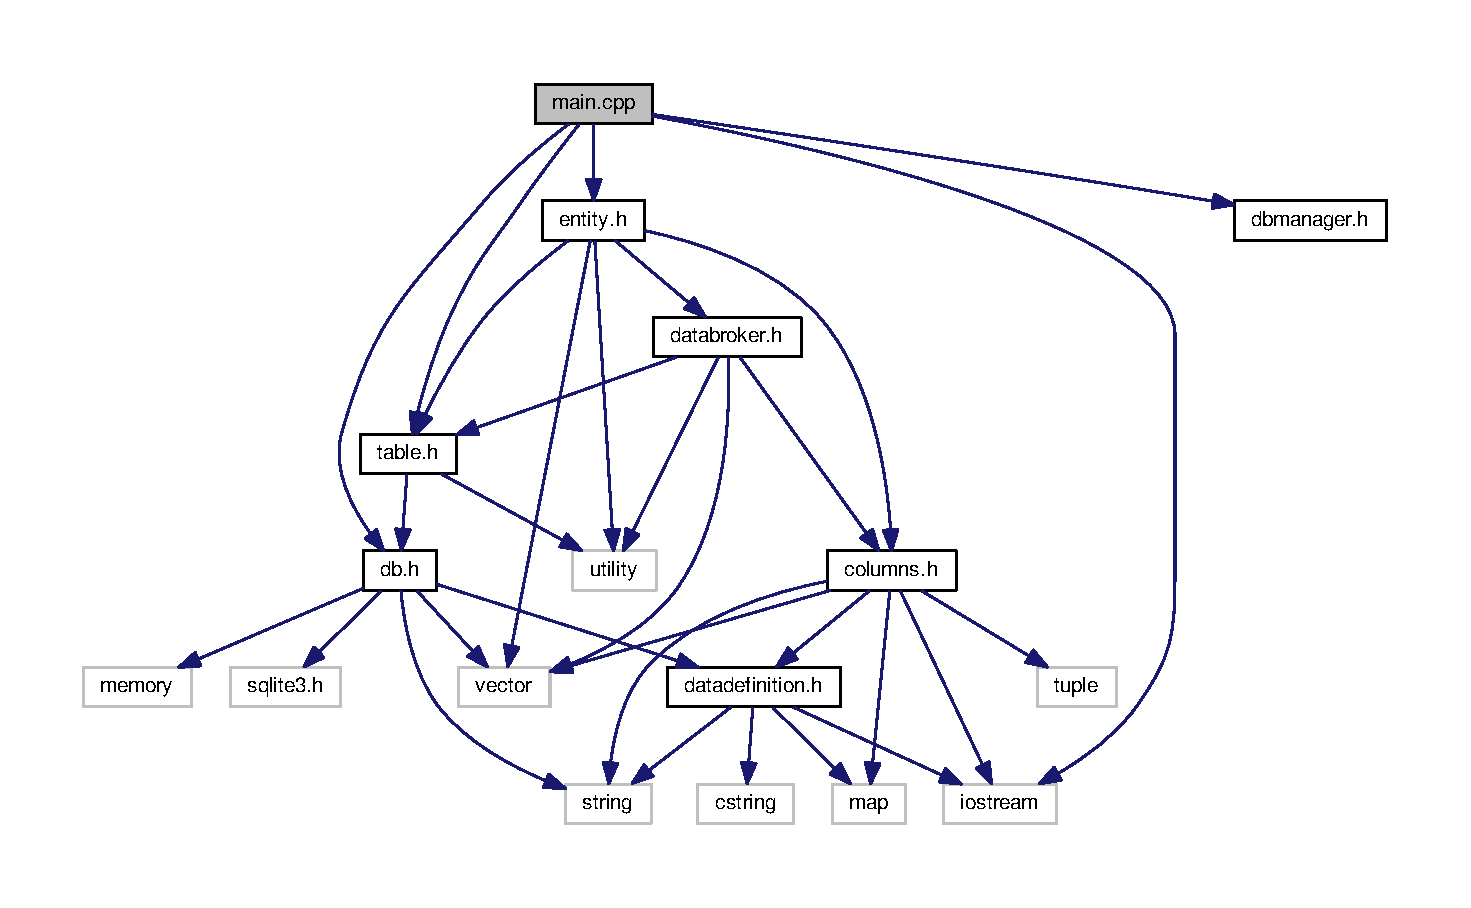
\includegraphics[width=350pt]{main_8cpp__incl}
\end{center}
\end{figure}
\subsection*{Classes}
\begin{DoxyCompactItemize}
\item 
class \mbox{\hyperlink{classUATData}{U\+A\+T\+Data}}
\item 
class \mbox{\hyperlink{classUATDomainCreationPolicy}{U\+A\+T\+Domain\+Creation\+Policy}}
\end{DoxyCompactItemize}
\subsection*{Typedefs}
\begin{DoxyCompactItemize}
\item 
typedef \mbox{\hyperlink{classDbManager}{Db\+Manager}}$<$ \mbox{\hyperlink{classUATDomainCreationPolicy}{U\+A\+T\+Domain\+Creation\+Policy}} $>$ \mbox{\hyperlink{main_8cpp_a22cf77c978c2d0de85bb8644ea6d100c}{U\+A\+T\+D\+B\+Manager}}
\end{DoxyCompactItemize}
\subsection*{Functions}
\begin{DoxyCompactItemize}
\item 
int \mbox{\hyperlink{main_8cpp_ae66f6b31b5ad750f1fe042a706a4e3d4}{main}} ()
\end{DoxyCompactItemize}


\subsection{Typedef Documentation}
\mbox{\Hypertarget{main_8cpp_a22cf77c978c2d0de85bb8644ea6d100c}\label{main_8cpp_a22cf77c978c2d0de85bb8644ea6d100c}} 
\index{main.\+cpp@{main.\+cpp}!U\+A\+T\+D\+B\+Manager@{U\+A\+T\+D\+B\+Manager}}
\index{U\+A\+T\+D\+B\+Manager@{U\+A\+T\+D\+B\+Manager}!main.\+cpp@{main.\+cpp}}
\subsubsection{\texorpdfstring{U\+A\+T\+D\+B\+Manager}{UATDBManager}}
{\footnotesize\ttfamily typedef \mbox{\hyperlink{classDbManager}{Db\+Manager}}$<$\mbox{\hyperlink{classUATDomainCreationPolicy}{U\+A\+T\+Domain\+Creation\+Policy}}$>$ \mbox{\hyperlink{main_8cpp_a22cf77c978c2d0de85bb8644ea6d100c}{U\+A\+T\+D\+B\+Manager}}}



\subsection{Function Documentation}
\mbox{\Hypertarget{main_8cpp_ae66f6b31b5ad750f1fe042a706a4e3d4}\label{main_8cpp_ae66f6b31b5ad750f1fe042a706a4e3d4}} 
\index{main.\+cpp@{main.\+cpp}!main@{main}}
\index{main@{main}!main.\+cpp@{main.\+cpp}}
\subsubsection{\texorpdfstring{main()}{main()}}
{\footnotesize\ttfamily int main (\begin{DoxyParamCaption}{ }\end{DoxyParamCaption})}

When creating an object, a singleton of D\+B\+Manager that follows a specific creation policy can be used. Such functions can also be shifted to a factory.
\hypertarget{README_8md}{}\section{R\+E\+A\+D\+M\+E.\+md File Reference}
\label{README_8md}\index{R\+E\+A\+D\+M\+E.\+md@{R\+E\+A\+D\+M\+E.\+md}}

\hypertarget{columns_8h}{}\section{sqlite-\/core/\+Headers/columns.h File Reference}
\label{columns_8h}\index{sqlite-\/core/\+Headers/columns.\+h@{sqlite-\/core/\+Headers/columns.\+h}}
{\ttfamily \#include $<$iostream$>$}\newline
{\ttfamily \#include $<$map$>$}\newline
{\ttfamily \#include $<$string$>$}\newline
{\ttfamily \#include $<$vector$>$}\newline
{\ttfamily \#include $<$tuple$>$}\newline
{\ttfamily \#include \char`\"{}datadefinition.\+h\char`\"{}}\newline
Include dependency graph for columns.\+h\+:\nopagebreak
\begin{figure}[H]
\begin{center}
\leavevmode
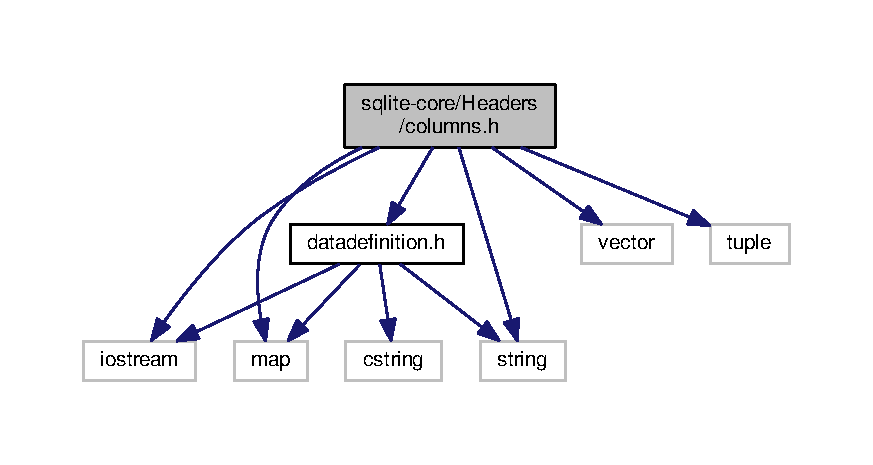
\includegraphics[width=350pt]{columns_8h__incl}
\end{center}
\end{figure}
This graph shows which files directly or indirectly include this file\+:\nopagebreak
\begin{figure}[H]
\begin{center}
\leavevmode
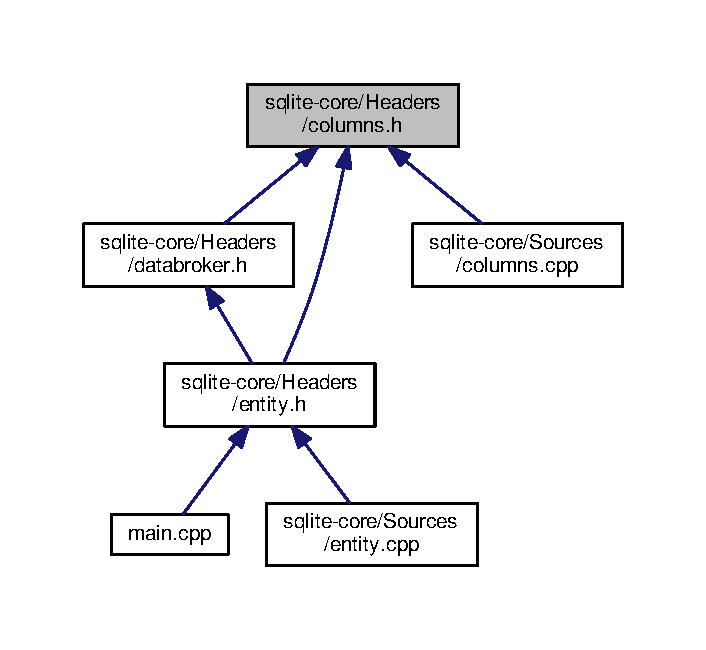
\includegraphics[width=339pt]{columns_8h__dep__incl}
\end{center}
\end{figure}
\subsection*{Classes}
\begin{DoxyCompactItemize}
\item 
class \mbox{\hyperlink{classColumns}{Columns}}
\end{DoxyCompactItemize}

\hypertarget{databroker_8h}{}\section{sqlite-\/core/\+Headers/databroker.h File Reference}
\label{databroker_8h}\index{sqlite-\/core/\+Headers/databroker.\+h@{sqlite-\/core/\+Headers/databroker.\+h}}
{\ttfamily \#include \char`\"{}table.\+h\char`\"{}}\newline
{\ttfamily \#include \char`\"{}columns.\+h\char`\"{}}\newline
{\ttfamily \#include $<$vector$>$}\newline
{\ttfamily \#include $<$utility$>$}\newline
Include dependency graph for databroker.\+h\+:\nopagebreak
\begin{figure}[H]
\begin{center}
\leavevmode
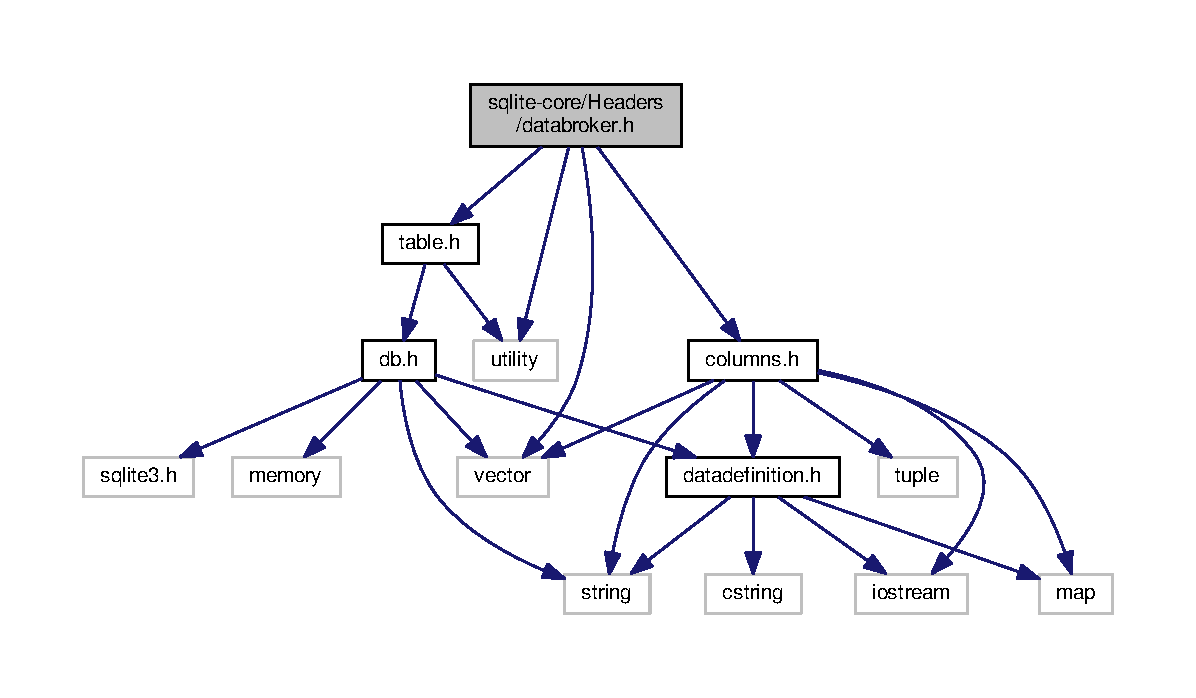
\includegraphics[width=350pt]{databroker_8h__incl}
\end{center}
\end{figure}
This graph shows which files directly or indirectly include this file\+:\nopagebreak
\begin{figure}[H]
\begin{center}
\leavevmode
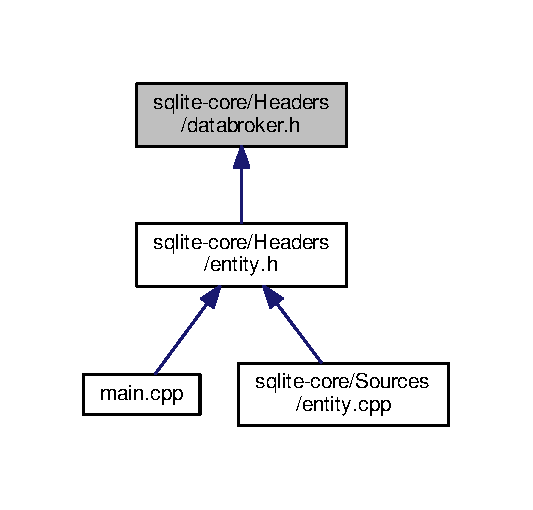
\includegraphics[width=256pt]{databroker_8h__dep__incl}
\end{center}
\end{figure}
\subsection*{Classes}
\begin{DoxyCompactItemize}
\item 
class \mbox{\hyperlink{classColumnsFromSqlValue}{Columns\+From\+Sql\+Value}}
\item 
class \mbox{\hyperlink{classSqlValueFromColumn}{Sql\+Value\+From\+Column}}
\end{DoxyCompactItemize}

\hypertarget{datadefinition_8h}{}\section{sqlite-\/core/\+Headers/datadefinition.h File Reference}
\label{datadefinition_8h}\index{sqlite-\/core/\+Headers/datadefinition.\+h@{sqlite-\/core/\+Headers/datadefinition.\+h}}
{\ttfamily \#include $<$string$>$}\newline
{\ttfamily \#include $<$iostream$>$}\newline
{\ttfamily \#include $<$cstring$>$}\newline
{\ttfamily \#include $<$map$>$}\newline
Include dependency graph for datadefinition.\+h\+:\nopagebreak
\begin{figure}[H]
\begin{center}
\leavevmode
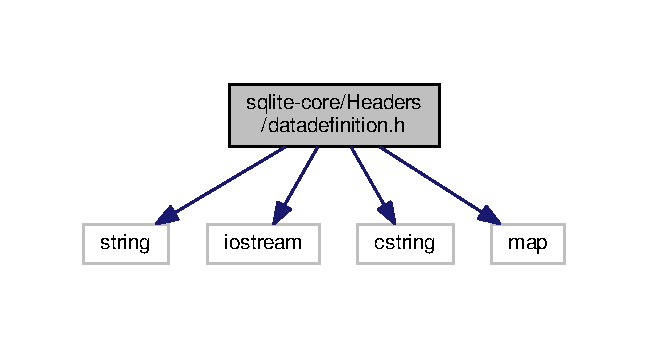
\includegraphics[width=311pt]{datadefinition_8h__incl}
\end{center}
\end{figure}
This graph shows which files directly or indirectly include this file\+:\nopagebreak
\begin{figure}[H]
\begin{center}
\leavevmode
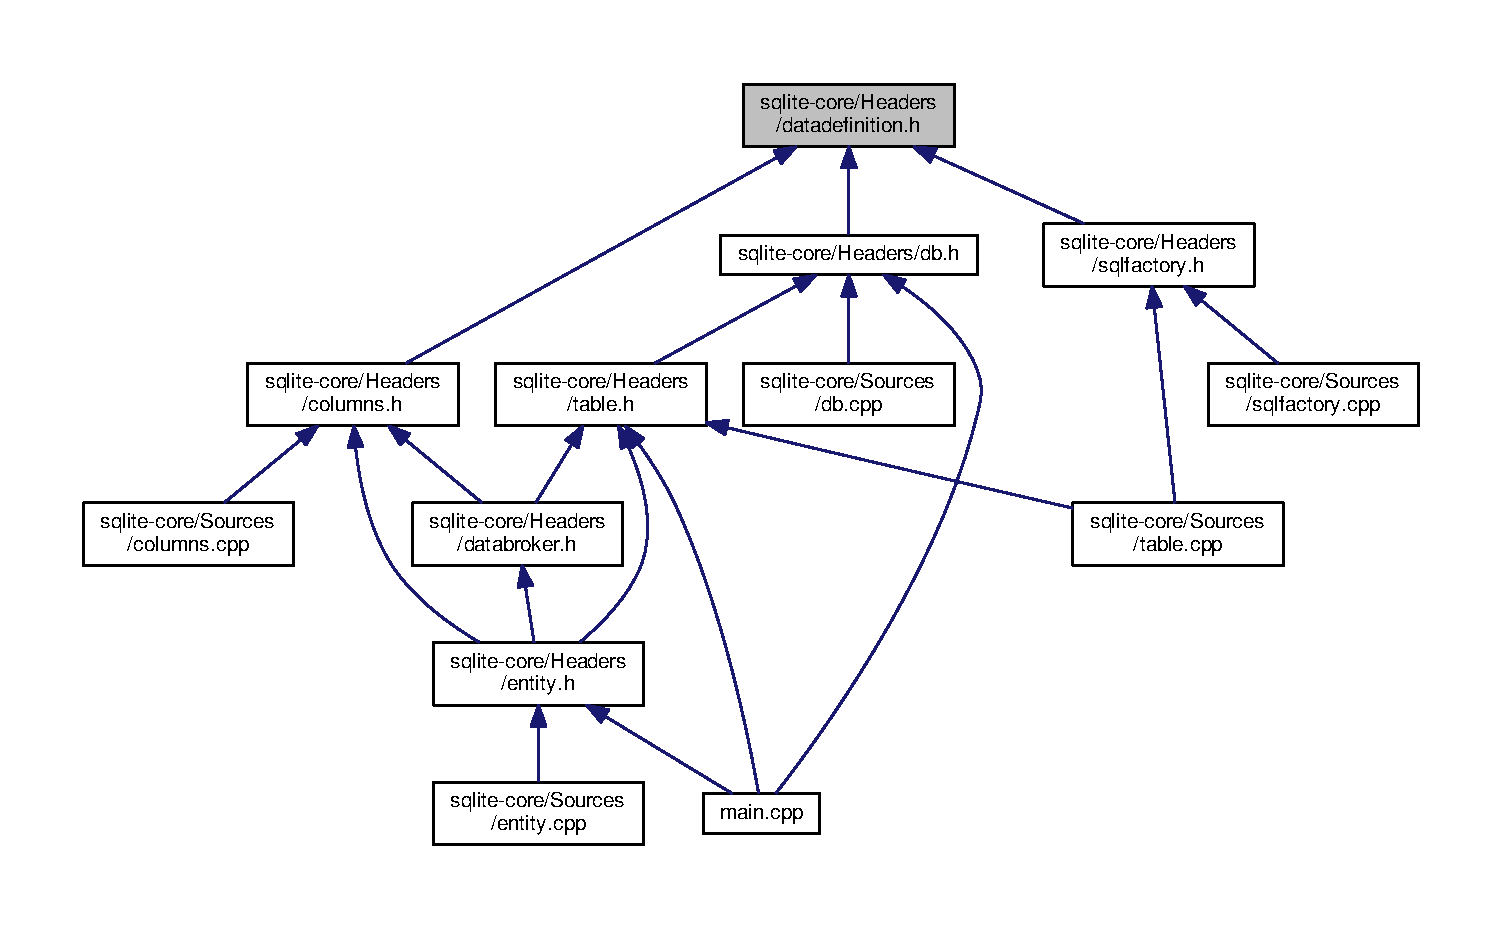
\includegraphics[width=350pt]{datadefinition_8h__dep__incl}
\end{center}
\end{figure}
\subsection*{Classes}
\begin{DoxyCompactItemize}
\item 
struct \mbox{\hyperlink{structSqlValue}{Sql\+Value}}
\item 
struct \mbox{\hyperlink{structSqlField}{Sql\+Field}}
\item 
struct \mbox{\hyperlink{structcmp__str}{cmp\+\_\+str}}
\end{DoxyCompactItemize}
\subsection*{Typedefs}
\begin{DoxyCompactItemize}
\item 
using \mbox{\hyperlink{datadefinition_8h_a09c0cd32f8797a9ad3df7daa788656cc}{map\+Sql\+Value}} = map$<$ const char $\ast$, \mbox{\hyperlink{structSqlValue}{Sql\+Value}}, \mbox{\hyperlink{structcmp__str}{cmp\+\_\+str}} $>$
\item 
using \mbox{\hyperlink{datadefinition_8h_aea73dfd4c959e6737c9c65474e4529ec}{map\+Int}} = map$<$ const char $\ast$, int, \mbox{\hyperlink{structcmp__str}{cmp\+\_\+str}} $>$
\item 
using \mbox{\hyperlink{datadefinition_8h_a9ada3c20f161f474bb963207a7f7bde5}{map\+Str}} = map$<$ const char $\ast$, string, \mbox{\hyperlink{structcmp__str}{cmp\+\_\+str}} $>$
\item 
using \mbox{\hyperlink{datadefinition_8h_aeaff661fb97ce7aa76f32e7e308f3a15}{map\+Float}} = map$<$ const char $\ast$, float, \mbox{\hyperlink{structcmp__str}{cmp\+\_\+str}} $>$
\item 
using \mbox{\hyperlink{datadefinition_8h_a143e5002d845b09ca5dcaf1eda71d70f}{map\+Bool}} = map$<$ const char $\ast$, bool, \mbox{\hyperlink{structcmp__str}{cmp\+\_\+str}} $>$
\item 
using \mbox{\hyperlink{datadefinition_8h_aec40b8d2d2c045d8af617ce94864651f}{schema}} = map$<$ const char $\ast$, \mbox{\hyperlink{datadefinition_8h_a5fcf79f0ca62a2c8a1c7f59c5974a485}{Platform\+Type\+Enum}}, \mbox{\hyperlink{structcmp__str}{cmp\+\_\+str}} $>$
\end{DoxyCompactItemize}
\subsection*{Enumerations}
\begin{DoxyCompactItemize}
\item 
enum \mbox{\hyperlink{datadefinition_8h_a5fcf79f0ca62a2c8a1c7f59c5974a485}{Platform\+Type\+Enum}} \{ \mbox{\hyperlink{datadefinition_8h_a5fcf79f0ca62a2c8a1c7f59c5974a485a34af25cf959804c283362a522fc7e804}{P\+L\+A\+T\+\_\+\+S\+TR}}, 
\mbox{\hyperlink{datadefinition_8h_a5fcf79f0ca62a2c8a1c7f59c5974a485a0f52b78bd2e4914c36bba4a853541f19}{P\+L\+A\+T\+\_\+\+I\+NT}}, 
\mbox{\hyperlink{datadefinition_8h_a5fcf79f0ca62a2c8a1c7f59c5974a485aad6c5381a50583862e50b7dac1c863b0}{P\+L\+A\+T\+\_\+\+D\+BL}}, 
\mbox{\hyperlink{datadefinition_8h_a5fcf79f0ca62a2c8a1c7f59c5974a485aa08eaaceff28a17eeb47c485308ecce5}{P\+L\+A\+T\+\_\+\+B\+O\+OL}}
 \}
\item 
enum \mbox{\hyperlink{datadefinition_8h_ad06ef517a8bb3398f146f81f18988b9f}{Sql\+Type\+Enum}} \{ \mbox{\hyperlink{datadefinition_8h_ad06ef517a8bb3398f146f81f18988b9faa5ec7b1f6f558b362f5a9ced5f228c2b}{S\+Q\+L\+\_\+\+S\+TR}}, 
\mbox{\hyperlink{datadefinition_8h_ad06ef517a8bb3398f146f81f18988b9fa460487fe5bd12482e12240aba6a08fae}{S\+Q\+L\+\_\+\+I\+NT}}, 
\mbox{\hyperlink{datadefinition_8h_ad06ef517a8bb3398f146f81f18988b9faf8e87d85b6cdee9030969a14f6ba011e}{S\+Q\+L\+\_\+\+D\+BL}}, 
\mbox{\hyperlink{datadefinition_8h_ad06ef517a8bb3398f146f81f18988b9fa4c175fbb65c723226d182dbfd556136a}{N\+UL}}
 \}
\end{DoxyCompactItemize}


\subsection{Typedef Documentation}
\mbox{\Hypertarget{datadefinition_8h_a143e5002d845b09ca5dcaf1eda71d70f}\label{datadefinition_8h_a143e5002d845b09ca5dcaf1eda71d70f}} 
\index{datadefinition.\+h@{datadefinition.\+h}!map\+Bool@{map\+Bool}}
\index{map\+Bool@{map\+Bool}!datadefinition.\+h@{datadefinition.\+h}}
\subsubsection{\texorpdfstring{map\+Bool}{mapBool}}
{\footnotesize\ttfamily using \mbox{\hyperlink{datadefinition_8h_a143e5002d845b09ca5dcaf1eda71d70f}{map\+Bool}} =  map$<$const char$\ast$, bool, \mbox{\hyperlink{structcmp__str}{cmp\+\_\+str}}$>$}

\mbox{\Hypertarget{datadefinition_8h_aeaff661fb97ce7aa76f32e7e308f3a15}\label{datadefinition_8h_aeaff661fb97ce7aa76f32e7e308f3a15}} 
\index{datadefinition.\+h@{datadefinition.\+h}!map\+Float@{map\+Float}}
\index{map\+Float@{map\+Float}!datadefinition.\+h@{datadefinition.\+h}}
\subsubsection{\texorpdfstring{map\+Float}{mapFloat}}
{\footnotesize\ttfamily using \mbox{\hyperlink{datadefinition_8h_aeaff661fb97ce7aa76f32e7e308f3a15}{map\+Float}} =  map$<$const char$\ast$, float, \mbox{\hyperlink{structcmp__str}{cmp\+\_\+str}}$>$}

\mbox{\Hypertarget{datadefinition_8h_aea73dfd4c959e6737c9c65474e4529ec}\label{datadefinition_8h_aea73dfd4c959e6737c9c65474e4529ec}} 
\index{datadefinition.\+h@{datadefinition.\+h}!map\+Int@{map\+Int}}
\index{map\+Int@{map\+Int}!datadefinition.\+h@{datadefinition.\+h}}
\subsubsection{\texorpdfstring{map\+Int}{mapInt}}
{\footnotesize\ttfamily using \mbox{\hyperlink{datadefinition_8h_aea73dfd4c959e6737c9c65474e4529ec}{map\+Int}} =  map$<$const char$\ast$, int, \mbox{\hyperlink{structcmp__str}{cmp\+\_\+str}}$>$}

\mbox{\Hypertarget{datadefinition_8h_a09c0cd32f8797a9ad3df7daa788656cc}\label{datadefinition_8h_a09c0cd32f8797a9ad3df7daa788656cc}} 
\index{datadefinition.\+h@{datadefinition.\+h}!map\+Sql\+Value@{map\+Sql\+Value}}
\index{map\+Sql\+Value@{map\+Sql\+Value}!datadefinition.\+h@{datadefinition.\+h}}
\subsubsection{\texorpdfstring{map\+Sql\+Value}{mapSqlValue}}
{\footnotesize\ttfamily using \mbox{\hyperlink{datadefinition_8h_a09c0cd32f8797a9ad3df7daa788656cc}{map\+Sql\+Value}} =  map$<$const char$\ast$, \mbox{\hyperlink{structSqlValue}{Sql\+Value}}, \mbox{\hyperlink{structcmp__str}{cmp\+\_\+str}}$>$}

\mbox{\Hypertarget{datadefinition_8h_a9ada3c20f161f474bb963207a7f7bde5}\label{datadefinition_8h_a9ada3c20f161f474bb963207a7f7bde5}} 
\index{datadefinition.\+h@{datadefinition.\+h}!map\+Str@{map\+Str}}
\index{map\+Str@{map\+Str}!datadefinition.\+h@{datadefinition.\+h}}
\subsubsection{\texorpdfstring{map\+Str}{mapStr}}
{\footnotesize\ttfamily using \mbox{\hyperlink{datadefinition_8h_a9ada3c20f161f474bb963207a7f7bde5}{map\+Str}} =  map$<$const char$\ast$, string, \mbox{\hyperlink{structcmp__str}{cmp\+\_\+str}}$>$}

\mbox{\Hypertarget{datadefinition_8h_aec40b8d2d2c045d8af617ce94864651f}\label{datadefinition_8h_aec40b8d2d2c045d8af617ce94864651f}} 
\index{datadefinition.\+h@{datadefinition.\+h}!schema@{schema}}
\index{schema@{schema}!datadefinition.\+h@{datadefinition.\+h}}
\subsubsection{\texorpdfstring{schema}{schema}}
{\footnotesize\ttfamily using \mbox{\hyperlink{datadefinition_8h_aec40b8d2d2c045d8af617ce94864651f}{schema}} =  map$<$const char$\ast$, \mbox{\hyperlink{datadefinition_8h_a5fcf79f0ca62a2c8a1c7f59c5974a485}{Platform\+Type\+Enum}}, \mbox{\hyperlink{structcmp__str}{cmp\+\_\+str}}$>$}



\subsection{Enumeration Type Documentation}
\mbox{\Hypertarget{datadefinition_8h_a5fcf79f0ca62a2c8a1c7f59c5974a485}\label{datadefinition_8h_a5fcf79f0ca62a2c8a1c7f59c5974a485}} 
\index{datadefinition.\+h@{datadefinition.\+h}!Platform\+Type\+Enum@{Platform\+Type\+Enum}}
\index{Platform\+Type\+Enum@{Platform\+Type\+Enum}!datadefinition.\+h@{datadefinition.\+h}}
\subsubsection{\texorpdfstring{Platform\+Type\+Enum}{PlatformTypeEnum}}
{\footnotesize\ttfamily enum \mbox{\hyperlink{datadefinition_8h_a5fcf79f0ca62a2c8a1c7f59c5974a485}{Platform\+Type\+Enum}}}

\begin{DoxyEnumFields}{Enumerator}
\raisebox{\heightof{T}}[0pt][0pt]{\index{P\+L\+A\+T\+\_\+\+S\+TR@{P\+L\+A\+T\+\_\+\+S\+TR}!datadefinition.\+h@{datadefinition.\+h}}\index{datadefinition.\+h@{datadefinition.\+h}!P\+L\+A\+T\+\_\+\+S\+TR@{P\+L\+A\+T\+\_\+\+S\+TR}}}\mbox{\Hypertarget{datadefinition_8h_a5fcf79f0ca62a2c8a1c7f59c5974a485a34af25cf959804c283362a522fc7e804}\label{datadefinition_8h_a5fcf79f0ca62a2c8a1c7f59c5974a485a34af25cf959804c283362a522fc7e804}} 
P\+L\+A\+T\+\_\+\+S\+TR&\\
\hline

\raisebox{\heightof{T}}[0pt][0pt]{\index{P\+L\+A\+T\+\_\+\+I\+NT@{P\+L\+A\+T\+\_\+\+I\+NT}!datadefinition.\+h@{datadefinition.\+h}}\index{datadefinition.\+h@{datadefinition.\+h}!P\+L\+A\+T\+\_\+\+I\+NT@{P\+L\+A\+T\+\_\+\+I\+NT}}}\mbox{\Hypertarget{datadefinition_8h_a5fcf79f0ca62a2c8a1c7f59c5974a485a0f52b78bd2e4914c36bba4a853541f19}\label{datadefinition_8h_a5fcf79f0ca62a2c8a1c7f59c5974a485a0f52b78bd2e4914c36bba4a853541f19}} 
P\+L\+A\+T\+\_\+\+I\+NT&\\
\hline

\raisebox{\heightof{T}}[0pt][0pt]{\index{P\+L\+A\+T\+\_\+\+D\+BL@{P\+L\+A\+T\+\_\+\+D\+BL}!datadefinition.\+h@{datadefinition.\+h}}\index{datadefinition.\+h@{datadefinition.\+h}!P\+L\+A\+T\+\_\+\+D\+BL@{P\+L\+A\+T\+\_\+\+D\+BL}}}\mbox{\Hypertarget{datadefinition_8h_a5fcf79f0ca62a2c8a1c7f59c5974a485aad6c5381a50583862e50b7dac1c863b0}\label{datadefinition_8h_a5fcf79f0ca62a2c8a1c7f59c5974a485aad6c5381a50583862e50b7dac1c863b0}} 
P\+L\+A\+T\+\_\+\+D\+BL&\\
\hline

\raisebox{\heightof{T}}[0pt][0pt]{\index{P\+L\+A\+T\+\_\+\+B\+O\+OL@{P\+L\+A\+T\+\_\+\+B\+O\+OL}!datadefinition.\+h@{datadefinition.\+h}}\index{datadefinition.\+h@{datadefinition.\+h}!P\+L\+A\+T\+\_\+\+B\+O\+OL@{P\+L\+A\+T\+\_\+\+B\+O\+OL}}}\mbox{\Hypertarget{datadefinition_8h_a5fcf79f0ca62a2c8a1c7f59c5974a485aa08eaaceff28a17eeb47c485308ecce5}\label{datadefinition_8h_a5fcf79f0ca62a2c8a1c7f59c5974a485aa08eaaceff28a17eeb47c485308ecce5}} 
P\+L\+A\+T\+\_\+\+B\+O\+OL&\\
\hline

\end{DoxyEnumFields}
\mbox{\Hypertarget{datadefinition_8h_ad06ef517a8bb3398f146f81f18988b9f}\label{datadefinition_8h_ad06ef517a8bb3398f146f81f18988b9f}} 
\index{datadefinition.\+h@{datadefinition.\+h}!Sql\+Type\+Enum@{Sql\+Type\+Enum}}
\index{Sql\+Type\+Enum@{Sql\+Type\+Enum}!datadefinition.\+h@{datadefinition.\+h}}
\subsubsection{\texorpdfstring{Sql\+Type\+Enum}{SqlTypeEnum}}
{\footnotesize\ttfamily enum \mbox{\hyperlink{datadefinition_8h_ad06ef517a8bb3398f146f81f18988b9f}{Sql\+Type\+Enum}}}

\begin{DoxyEnumFields}{Enumerator}
\raisebox{\heightof{T}}[0pt][0pt]{\index{S\+Q\+L\+\_\+\+S\+TR@{S\+Q\+L\+\_\+\+S\+TR}!datadefinition.\+h@{datadefinition.\+h}}\index{datadefinition.\+h@{datadefinition.\+h}!S\+Q\+L\+\_\+\+S\+TR@{S\+Q\+L\+\_\+\+S\+TR}}}\mbox{\Hypertarget{datadefinition_8h_ad06ef517a8bb3398f146f81f18988b9faa5ec7b1f6f558b362f5a9ced5f228c2b}\label{datadefinition_8h_ad06ef517a8bb3398f146f81f18988b9faa5ec7b1f6f558b362f5a9ced5f228c2b}} 
S\+Q\+L\+\_\+\+S\+TR&\\
\hline

\raisebox{\heightof{T}}[0pt][0pt]{\index{S\+Q\+L\+\_\+\+I\+NT@{S\+Q\+L\+\_\+\+I\+NT}!datadefinition.\+h@{datadefinition.\+h}}\index{datadefinition.\+h@{datadefinition.\+h}!S\+Q\+L\+\_\+\+I\+NT@{S\+Q\+L\+\_\+\+I\+NT}}}\mbox{\Hypertarget{datadefinition_8h_ad06ef517a8bb3398f146f81f18988b9fa460487fe5bd12482e12240aba6a08fae}\label{datadefinition_8h_ad06ef517a8bb3398f146f81f18988b9fa460487fe5bd12482e12240aba6a08fae}} 
S\+Q\+L\+\_\+\+I\+NT&\\
\hline

\raisebox{\heightof{T}}[0pt][0pt]{\index{S\+Q\+L\+\_\+\+D\+BL@{S\+Q\+L\+\_\+\+D\+BL}!datadefinition.\+h@{datadefinition.\+h}}\index{datadefinition.\+h@{datadefinition.\+h}!S\+Q\+L\+\_\+\+D\+BL@{S\+Q\+L\+\_\+\+D\+BL}}}\mbox{\Hypertarget{datadefinition_8h_ad06ef517a8bb3398f146f81f18988b9faf8e87d85b6cdee9030969a14f6ba011e}\label{datadefinition_8h_ad06ef517a8bb3398f146f81f18988b9faf8e87d85b6cdee9030969a14f6ba011e}} 
S\+Q\+L\+\_\+\+D\+BL&\\
\hline

\raisebox{\heightof{T}}[0pt][0pt]{\index{N\+UL@{N\+UL}!datadefinition.\+h@{datadefinition.\+h}}\index{datadefinition.\+h@{datadefinition.\+h}!N\+UL@{N\+UL}}}\mbox{\Hypertarget{datadefinition_8h_ad06ef517a8bb3398f146f81f18988b9fa4c175fbb65c723226d182dbfd556136a}\label{datadefinition_8h_ad06ef517a8bb3398f146f81f18988b9fa4c175fbb65c723226d182dbfd556136a}} 
N\+UL&\\
\hline

\end{DoxyEnumFields}

\hypertarget{db_8h}{}\section{sqlite-\/core/\+Headers/db.h File Reference}
\label{db_8h}\index{sqlite-\/core/\+Headers/db.\+h@{sqlite-\/core/\+Headers/db.\+h}}
{\ttfamily \#include $<$sqlite3.\+h$>$}\newline
{\ttfamily \#include $<$memory$>$}\newline
{\ttfamily \#include $<$vector$>$}\newline
{\ttfamily \#include $<$string$>$}\newline
{\ttfamily \#include \char`\"{}datadefinition.\+h\char`\"{}}\newline
Include dependency graph for db.\+h\+:\nopagebreak
\begin{figure}[H]
\begin{center}
\leavevmode
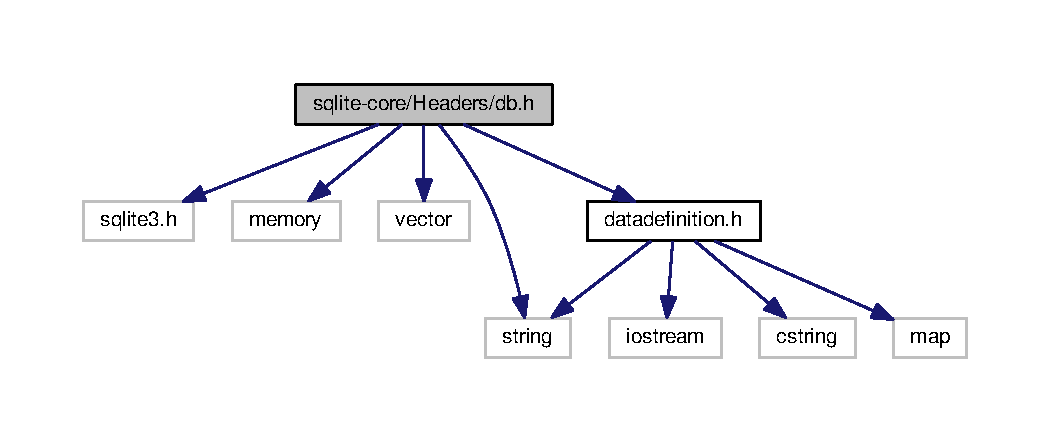
\includegraphics[width=350pt]{db_8h__incl}
\end{center}
\end{figure}
This graph shows which files directly or indirectly include this file\+:\nopagebreak
\begin{figure}[H]
\begin{center}
\leavevmode
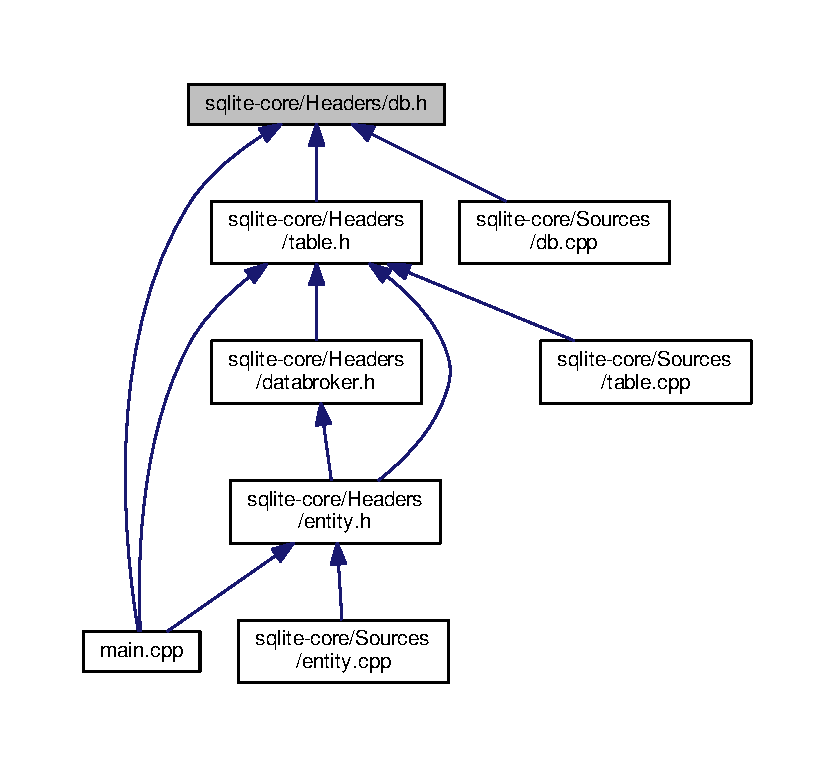
\includegraphics[width=350pt]{db_8h__dep__incl}
\end{center}
\end{figure}
\subsection*{Classes}
\begin{DoxyCompactItemize}
\item 
struct \mbox{\hyperlink{structsqlite3__deleter}{sqlite3\+\_\+deleter}}
\item 
struct \mbox{\hyperlink{structsqlite3__stmt__deleter}{sqlite3\+\_\+stmt\+\_\+deleter}}
\item 
class \mbox{\hyperlink{classDB}{DB}}
\end{DoxyCompactItemize}
\subsection*{Typedefs}
\begin{DoxyCompactItemize}
\item 
using \mbox{\hyperlink{db_8h_a8c50929ef9b94683ef6653b885e5b9ed}{sqldb}} = std\+::unique\+\_\+ptr$<$ sqlite3, \mbox{\hyperlink{structsqlite3__deleter}{sqlite3\+\_\+deleter}} $>$
\item 
using \mbox{\hyperlink{db_8h_a9c9e9eb73219858e1bd90c84d44e9728}{sqlstmt}} = std\+::unique\+\_\+ptr$<$ sqlite3\+\_\+stmt, \mbox{\hyperlink{structsqlite3__stmt__deleter}{sqlite3\+\_\+stmt\+\_\+deleter}} $>$
\item 
using \mbox{\hyperlink{db_8h_a356f4bbcc8528145c25584033ef0bcb8}{sql\+Result}} = std\+::vector$<$ std\+::vector$<$ \mbox{\hyperlink{structSqlValue}{Sql\+Value}} $>$ $>$
\end{DoxyCompactItemize}


\subsection{Typedef Documentation}
\mbox{\Hypertarget{db_8h_a8c50929ef9b94683ef6653b885e5b9ed}\label{db_8h_a8c50929ef9b94683ef6653b885e5b9ed}} 
\index{db.\+h@{db.\+h}!sqldb@{sqldb}}
\index{sqldb@{sqldb}!db.\+h@{db.\+h}}
\subsubsection{\texorpdfstring{sqldb}{sqldb}}
{\footnotesize\ttfamily using \mbox{\hyperlink{db_8h_a8c50929ef9b94683ef6653b885e5b9ed}{sqldb}} =  std\+::unique\+\_\+ptr$<$sqlite3, \mbox{\hyperlink{structsqlite3__deleter}{sqlite3\+\_\+deleter}}$>$}

\mbox{\Hypertarget{db_8h_a356f4bbcc8528145c25584033ef0bcb8}\label{db_8h_a356f4bbcc8528145c25584033ef0bcb8}} 
\index{db.\+h@{db.\+h}!sql\+Result@{sql\+Result}}
\index{sql\+Result@{sql\+Result}!db.\+h@{db.\+h}}
\subsubsection{\texorpdfstring{sql\+Result}{sqlResult}}
{\footnotesize\ttfamily using \mbox{\hyperlink{db_8h_a356f4bbcc8528145c25584033ef0bcb8}{sql\+Result}} =  std\+::vector$<$std\+::vector$<$\mbox{\hyperlink{structSqlValue}{Sql\+Value}}$>$ $>$}

\mbox{\Hypertarget{db_8h_a9c9e9eb73219858e1bd90c84d44e9728}\label{db_8h_a9c9e9eb73219858e1bd90c84d44e9728}} 
\index{db.\+h@{db.\+h}!sqlstmt@{sqlstmt}}
\index{sqlstmt@{sqlstmt}!db.\+h@{db.\+h}}
\subsubsection{\texorpdfstring{sqlstmt}{sqlstmt}}
{\footnotesize\ttfamily using \mbox{\hyperlink{db_8h_a9c9e9eb73219858e1bd90c84d44e9728}{sqlstmt}} =  std\+::unique\+\_\+ptr$<$sqlite3\+\_\+stmt, \mbox{\hyperlink{structsqlite3__stmt__deleter}{sqlite3\+\_\+stmt\+\_\+deleter}}$>$}


\hypertarget{dbmanager_8h}{}\section{sqlite-\/core/\+Headers/dbmanager.h File Reference}
\label{dbmanager_8h}\index{sqlite-\/core/\+Headers/dbmanager.\+h@{sqlite-\/core/\+Headers/dbmanager.\+h}}
This graph shows which files directly or indirectly include this file\+:\nopagebreak
\begin{figure}[H]
\begin{center}
\leavevmode
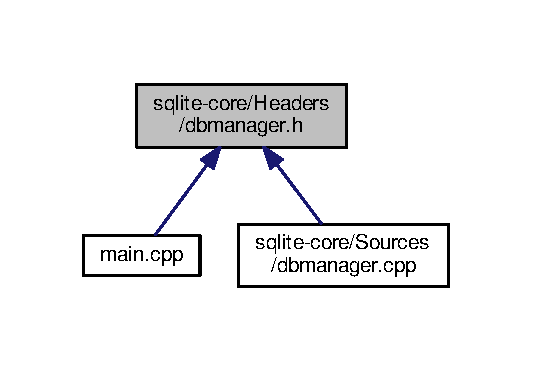
\includegraphics[width=256pt]{dbmanager_8h__dep__incl}
\end{center}
\end{figure}
\subsection*{Classes}
\begin{DoxyCompactItemize}
\item 
class \mbox{\hyperlink{classDefaultDataCreationPolicy}{Default\+Data\+Creation\+Policy}}
\item 
class \mbox{\hyperlink{classDbManager}{Db\+Manager$<$ Entity\+Creation\+Policy $>$}}
\end{DoxyCompactItemize}

\hypertarget{entity_8h}{}\section{sqlite-\/core/\+Headers/entity.h File Reference}
\label{entity_8h}\index{sqlite-\/core/\+Headers/entity.\+h@{sqlite-\/core/\+Headers/entity.\+h}}
{\ttfamily \#include \char`\"{}table.\+h\char`\"{}}\newline
{\ttfamily \#include \char`\"{}columns.\+h\char`\"{}}\newline
{\ttfamily \#include $<$vector$>$}\newline
{\ttfamily \#include $<$utility$>$}\newline
{\ttfamily \#include \char`\"{}databroker.\+h\char`\"{}}\newline
Include dependency graph for entity.\+h\+:\nopagebreak
\begin{figure}[H]
\begin{center}
\leavevmode
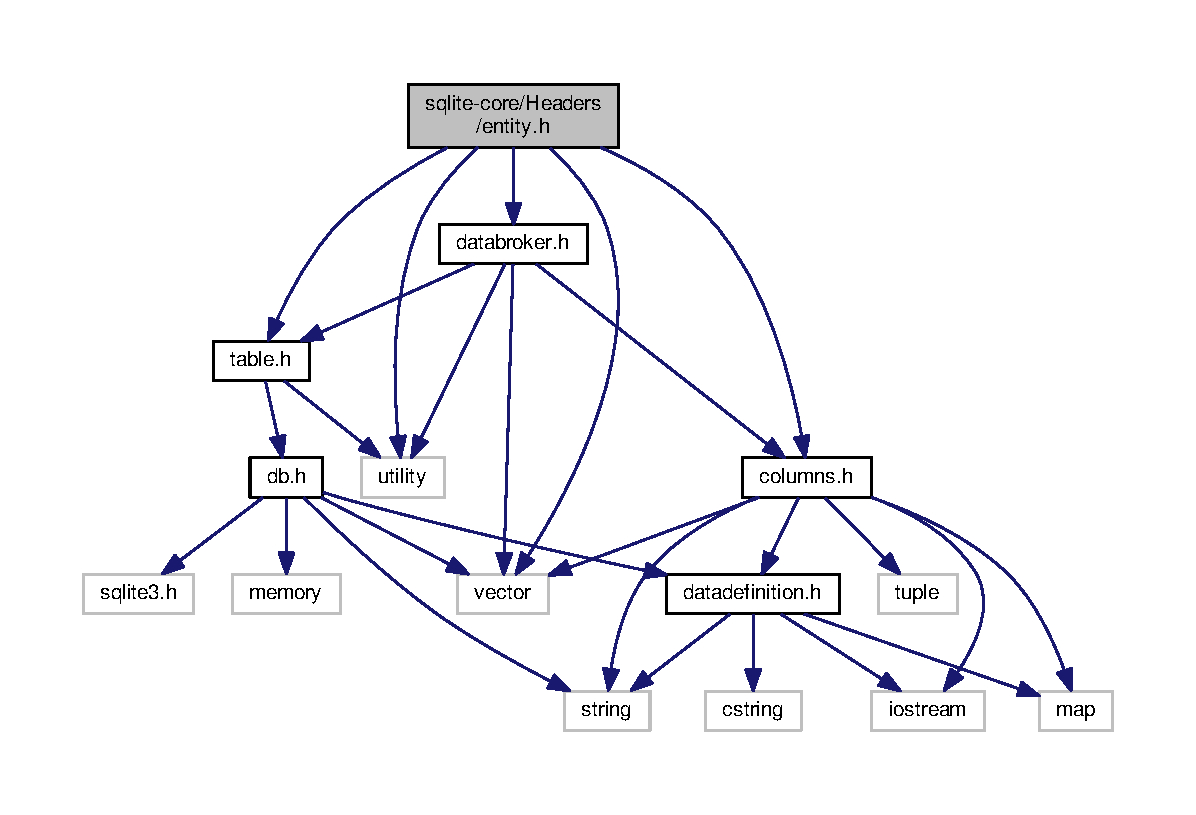
\includegraphics[width=350pt]{entity_8h__incl}
\end{center}
\end{figure}
This graph shows which files directly or indirectly include this file\+:\nopagebreak
\begin{figure}[H]
\begin{center}
\leavevmode
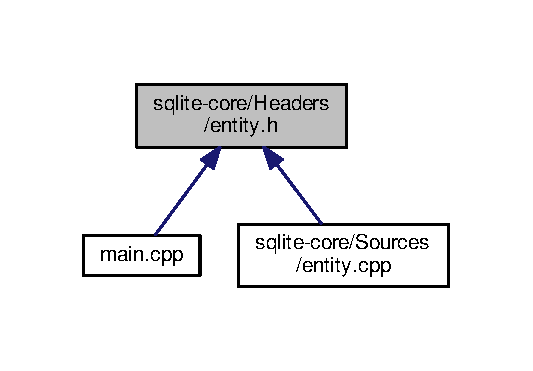
\includegraphics[width=256pt]{entity_8h__dep__incl}
\end{center}
\end{figure}
\subsection*{Classes}
\begin{DoxyCompactItemize}
\item 
class \mbox{\hyperlink{classEntity}{Entity}}
\end{DoxyCompactItemize}

\hypertarget{sqlfactory_8h}{}\section{sqlite-\/core/\+Headers/sqlfactory.h File Reference}
\label{sqlfactory_8h}\index{sqlite-\/core/\+Headers/sqlfactory.\+h@{sqlite-\/core/\+Headers/sqlfactory.\+h}}
{\ttfamily \#include $<$iostream$>$}\newline
{\ttfamily \#include $<$sstream$>$}\newline
{\ttfamily \#include $<$string$>$}\newline
{\ttfamily \#include $<$cstdio$>$}\newline
{\ttfamily \#include $<$utility$>$}\newline
{\ttfamily \#include $<$vector$>$}\newline
{\ttfamily \#include \char`\"{}datadefinition.\+h\char`\"{}}\newline
Include dependency graph for sqlfactory.\+h\+:\nopagebreak
\begin{figure}[H]
\begin{center}
\leavevmode
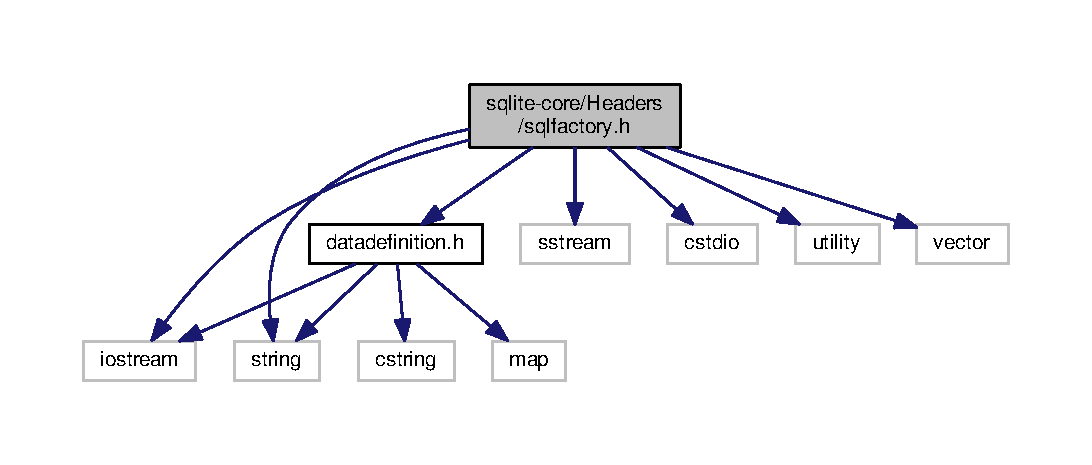
\includegraphics[width=350pt]{sqlfactory_8h__incl}
\end{center}
\end{figure}
This graph shows which files directly or indirectly include this file\+:\nopagebreak
\begin{figure}[H]
\begin{center}
\leavevmode
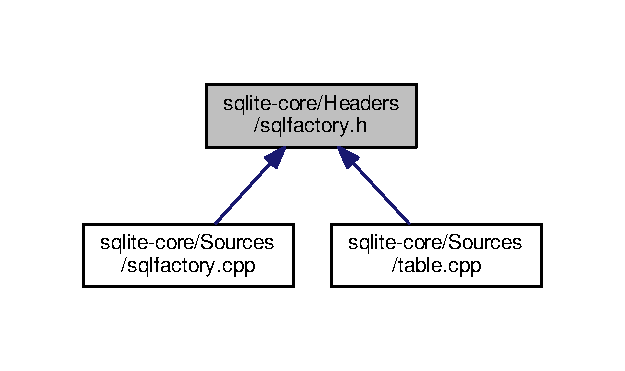
\includegraphics[width=300pt]{sqlfactory_8h__dep__incl}
\end{center}
\end{figure}
\subsection*{Classes}
\begin{DoxyCompactItemize}
\item 
class \mbox{\hyperlink{classSqlFactory}{Sql\+Factory}}
\end{DoxyCompactItemize}

\hypertarget{table_8h}{}\section{sqlite-\/core/\+Headers/table.h File Reference}
\label{table_8h}\index{sqlite-\/core/\+Headers/table.\+h@{sqlite-\/core/\+Headers/table.\+h}}
{\ttfamily \#include \char`\"{}db.\+h\char`\"{}}\newline
{\ttfamily \#include $<$utility$>$}\newline
Include dependency graph for table.\+h\+:\nopagebreak
\begin{figure}[H]
\begin{center}
\leavevmode
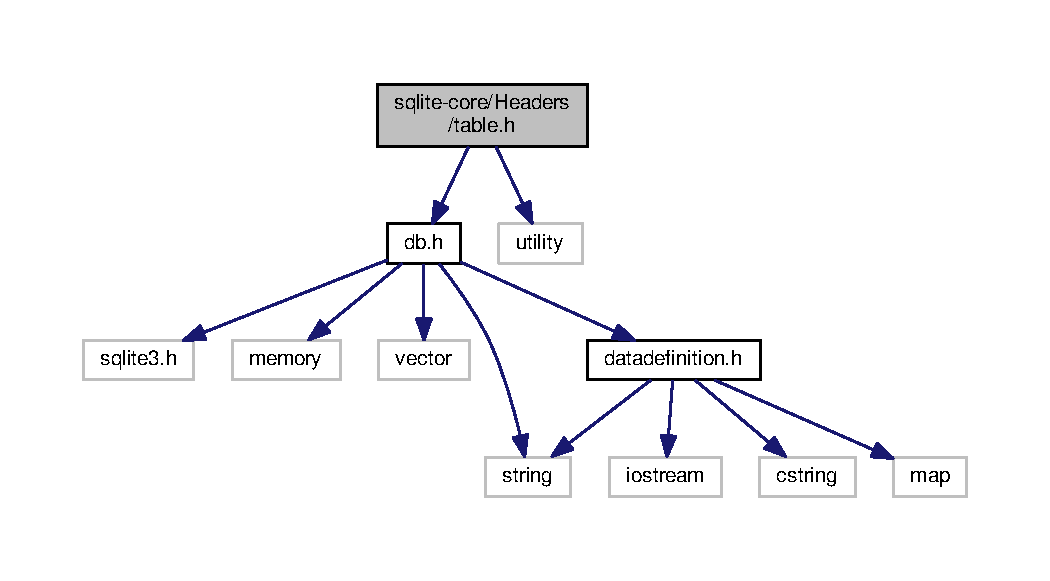
\includegraphics[width=350pt]{table_8h__incl}
\end{center}
\end{figure}
This graph shows which files directly or indirectly include this file\+:\nopagebreak
\begin{figure}[H]
\begin{center}
\leavevmode
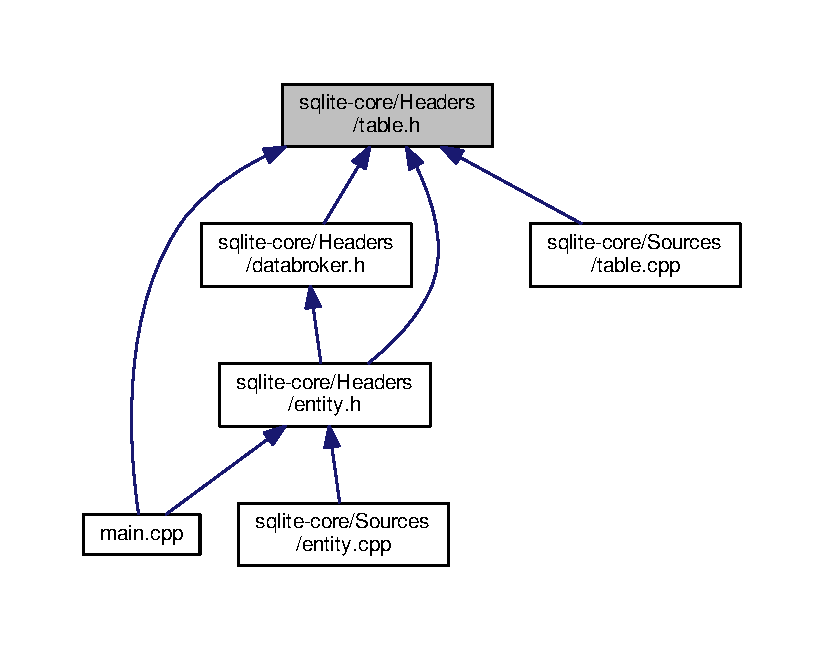
\includegraphics[width=350pt]{table_8h__dep__incl}
\end{center}
\end{figure}
\subsection*{Classes}
\begin{DoxyCompactItemize}
\item 
class \mbox{\hyperlink{classTable}{Table}}
\end{DoxyCompactItemize}

\hypertarget{columns_8cpp}{}\section{sqlite-\/core/\+Sources/columns.cpp File Reference}
\label{columns_8cpp}\index{sqlite-\/core/\+Sources/columns.\+cpp@{sqlite-\/core/\+Sources/columns.\+cpp}}
{\ttfamily \#include \char`\"{}columns.\+h\char`\"{}}\newline
Include dependency graph for columns.\+cpp\+:\nopagebreak
\begin{figure}[H]
\begin{center}
\leavevmode
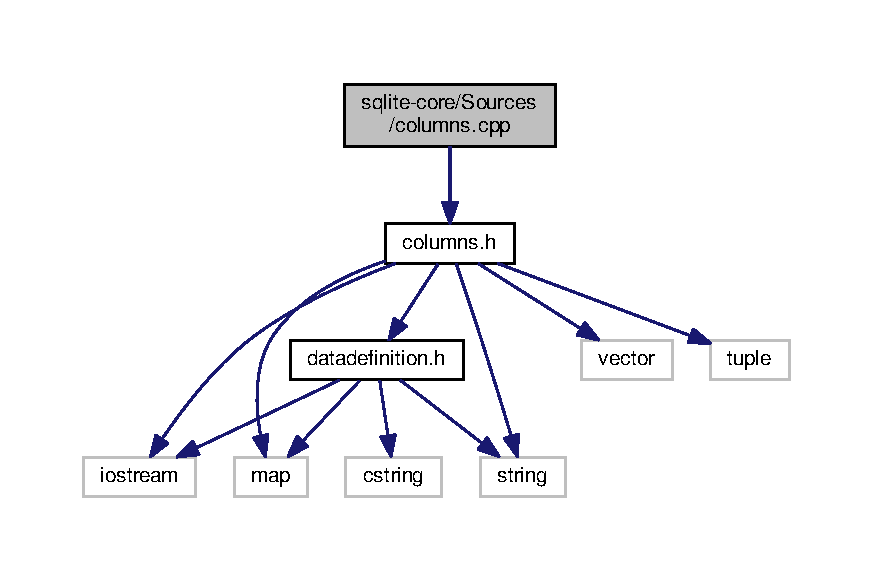
\includegraphics[width=350pt]{columns_8cpp__incl}
\end{center}
\end{figure}

\hypertarget{db_8cpp}{}\section{sqlite-\/core/\+Sources/db.cpp File Reference}
\label{db_8cpp}\index{sqlite-\/core/\+Sources/db.\+cpp@{sqlite-\/core/\+Sources/db.\+cpp}}
{\ttfamily \#include \char`\"{}db.\+h\char`\"{}}\newline
{\ttfamily \#include $<$sqlite3.\+h$>$}\newline
{\ttfamily \#include $<$stdio.\+h$>$}\newline
{\ttfamily \#include $<$memory$>$}\newline
{\ttfamily \#include $<$string.\+h$>$}\newline
Include dependency graph for db.\+cpp\+:\nopagebreak
\begin{figure}[H]
\begin{center}
\leavevmode
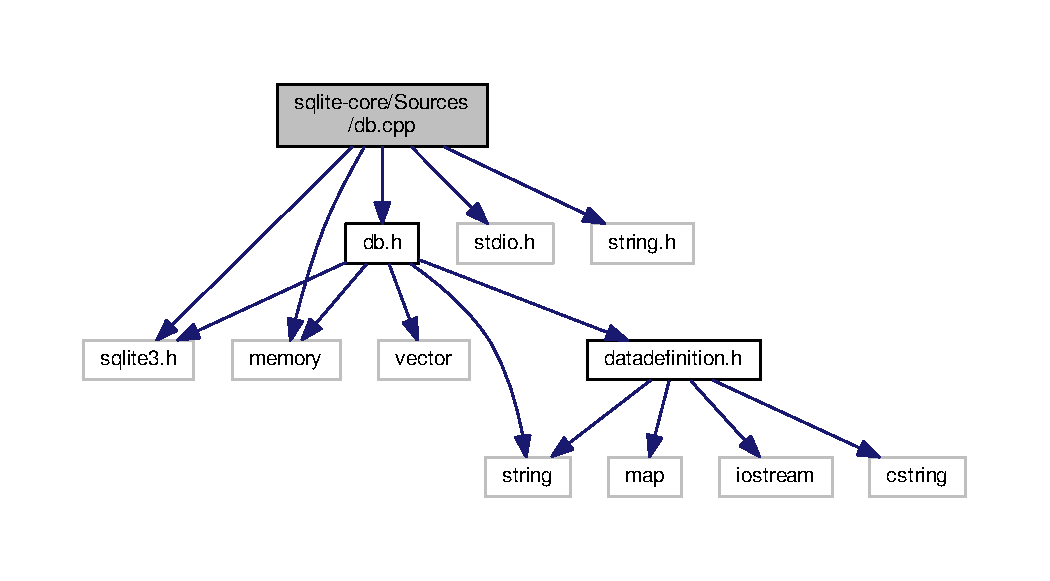
\includegraphics[width=350pt]{db_8cpp__incl}
\end{center}
\end{figure}

\hypertarget{dbmanager_8cpp}{}\section{sqlite-\/core/\+Sources/dbmanager.cpp File Reference}
\label{dbmanager_8cpp}\index{sqlite-\/core/\+Sources/dbmanager.\+cpp@{sqlite-\/core/\+Sources/dbmanager.\+cpp}}
{\ttfamily \#include \char`\"{}dbmanager.\+h\char`\"{}}\newline
Include dependency graph for dbmanager.\+cpp\+:\nopagebreak
\begin{figure}[H]
\begin{center}
\leavevmode
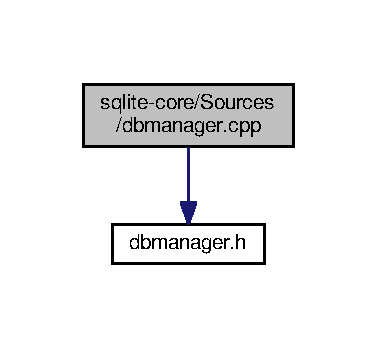
\includegraphics[width=181pt]{dbmanager_8cpp__incl}
\end{center}
\end{figure}

\hypertarget{entity_8cpp}{}\section{sqlite-\/core/\+Sources/entity.cpp File Reference}
\label{entity_8cpp}\index{sqlite-\/core/\+Sources/entity.\+cpp@{sqlite-\/core/\+Sources/entity.\+cpp}}
{\ttfamily \#include \char`\"{}entity.\+h\char`\"{}}\newline
Include dependency graph for entity.\+cpp\+:\nopagebreak
\begin{figure}[H]
\begin{center}
\leavevmode
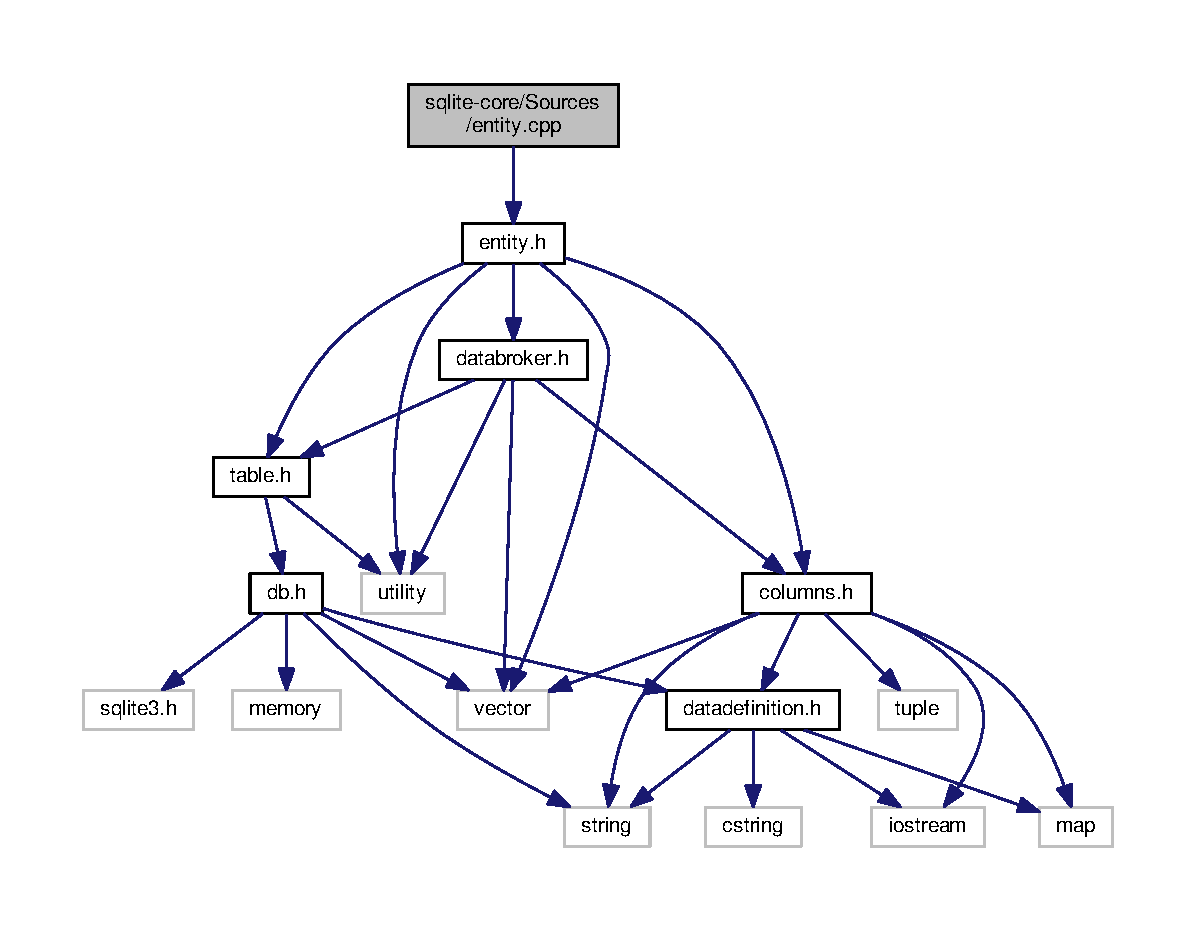
\includegraphics[width=350pt]{entity_8cpp__incl}
\end{center}
\end{figure}

\hypertarget{sqlfactory_8cpp}{}\section{sqlite-\/core/\+Sources/sqlfactory.cpp File Reference}
\label{sqlfactory_8cpp}\index{sqlite-\/core/\+Sources/sqlfactory.\+cpp@{sqlite-\/core/\+Sources/sqlfactory.\+cpp}}
{\ttfamily \#include \char`\"{}sqlfactory.\+h\char`\"{}}\newline
{\ttfamily \#include $<$vector$>$}\newline
Include dependency graph for sqlfactory.\+cpp\+:\nopagebreak
\begin{figure}[H]
\begin{center}
\leavevmode
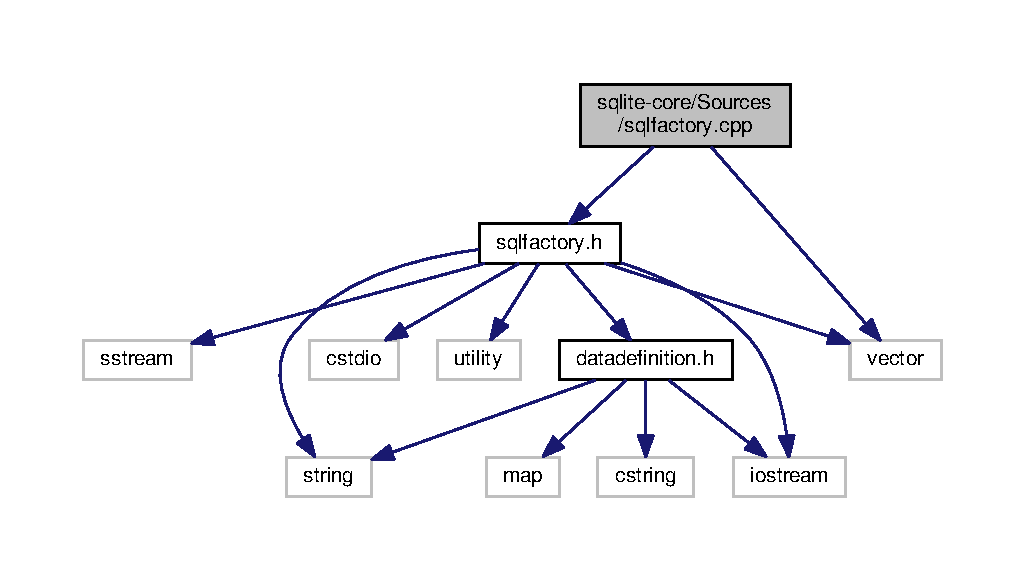
\includegraphics[width=350pt]{sqlfactory_8cpp__incl}
\end{center}
\end{figure}

\hypertarget{table_8cpp}{}\section{sqlite-\/core/\+Sources/table.cpp File Reference}
\label{table_8cpp}\index{sqlite-\/core/\+Sources/table.\+cpp@{sqlite-\/core/\+Sources/table.\+cpp}}
{\ttfamily \#include \char`\"{}table.\+h\char`\"{}}\newline
{\ttfamily \#include \char`\"{}sqlfactory.\+h\char`\"{}}\newline
{\ttfamily \#include $<$cmath$>$}\newline
Include dependency graph for table.\+cpp\+:\nopagebreak
\begin{figure}[H]
\begin{center}
\leavevmode
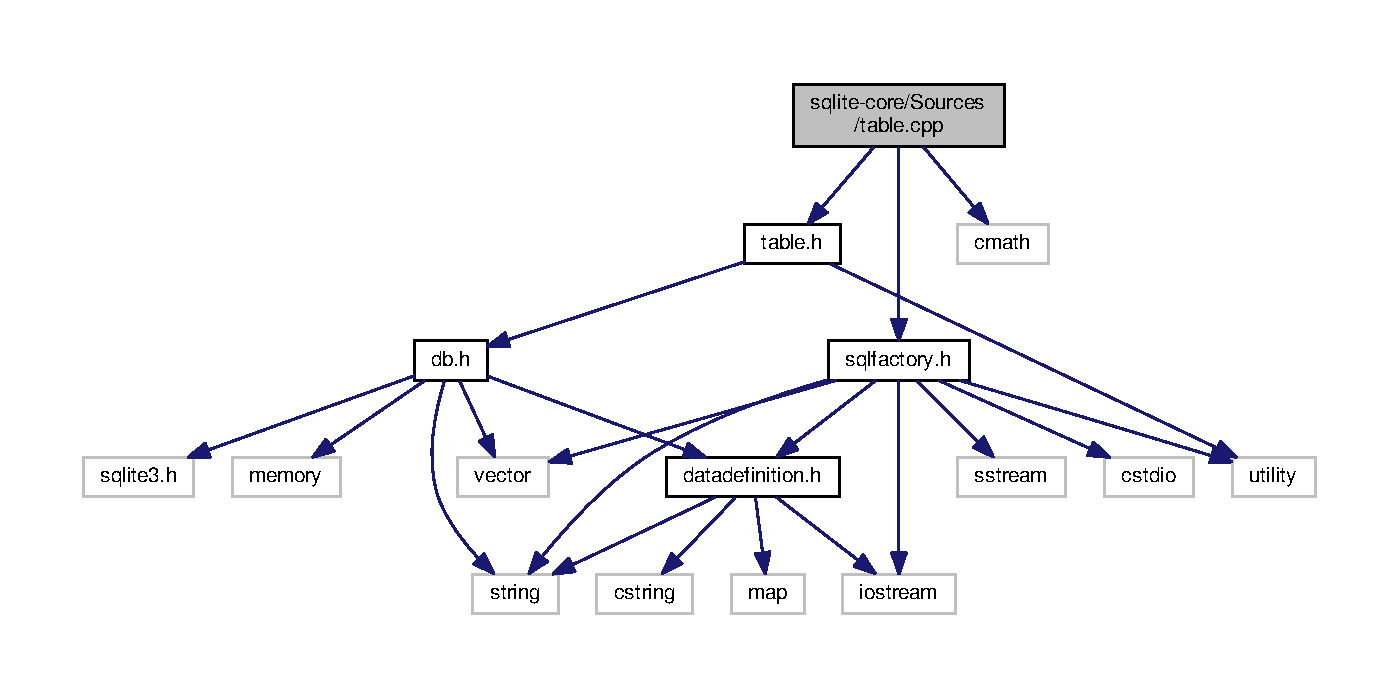
\includegraphics[width=350pt]{table_8cpp__incl}
\end{center}
\end{figure}

%--- End generated contents ---

% Index
\backmatter
\newpage
\phantomsection
\clearemptydoublepage
\addcontentsline{toc}{chapter}{Index}
\printindex

\end{document}
